%% Put these somewhwere:

\XXX{use svalue(g), spacing to give some breathing room in a ggroup}

\XXX{something like ggroup(cont=w,spacing=10); svalue(g)=10}

\XXX{include listing data frame, listing variables by type}

\XXX{relationship with the toolkits

\XXX{getToolkitWidget, add method, ... only with RGtk2 (rJava?), only some widgets}}



%% gWidgets introduction
 
\newcommand{\ONLYIN}[1]{[only in #1]}

\chapter{\pkg{gWidgets}: Overview}
\label{sec:overview}

%% Overview of gWidgets

The \pkg{gWidgets} package provides a toolkit-independent
interface for the \R\/ user to program graphical user interfaces from
within R. Although the package provides much less functionality than using the
native toolkits through their \R\/ bindings,  \pkg{gWidgets}  can be used to create moderately large
GUIs quickly and easily using a programming interface that is simpler and familiar for the \R\/ user
to learn.

 
The \pkg{gWidgets} package started as a port to \pkg{RGtk2}
of the \pkg{iWidgets} interface for \pkg{rJava}~\citep{iWidgets}. The
\pkg{gWidgets} package  enhances that original interface in
terms of functionality and is now toolkit independent.


\section{Installation, toolkits}
\label{sec:installation}

The \pkg{gWidgets} package is installed and loaded as other \R\/
packages that reside on CRAN. This can be done through the function
\code{install.packages} or on some OSes through a dialog called from
the menu bar. The \pkg{gWidgets} package provides the programming interface only (API). To
actually create a GUI, one needs to have the underlying toolkit libraries, an
underlying \R\/ package that provides an interface to the libraries,
and a \pkg{gWidgetsXXX} package to link \pkg{gWidgets} to the \R\/
package. The installation of the libraries varies depending on toolkit
and OS. Some details are presented by the function
\code{installing\_gWidgets\_toolkits}. 

As of this writing, there are basically complete \pkg{gWidgets}
packages for the toolkit packages \pkg{RGtk2} and \pkg{tcltk};
\pkg{gWidgetsWWW} ports the API to allow interactive web pages
(cf. Chapter~\ref{chap:WebGUIS}). Also there is \pkg{gWidgetsrJava},
but that package is not being supported. Here, only the
implementations for the \pkg{RGtk2} and \pkg{tcltk} packages are
covered.

Not all features of the API are available in each package.  The help
pages in \pkg{gWidgets} describe the API, with the help pages in the
toolkit packages indicating differences or omissions from the API. For
the most part, the omissions are gracefully handled by simply
providing less functionality. We make note of these differences for
\pkg{gWidgetsRGtk2} and \pkg{gWidgetstcltk} here, realizing that over
time they may may be resolved. Consult the package documentation if in
doubt.

Figure~\ref{fig:gWidgets-three-oses} shows how the same GUI code
can be rendered differently depending on the OS and the
toolkit. 

%%Figure~\ref{fig:gWidgetsWWW-same-gui} shows a similar GUI
%%using \pkg{gWidgetsWWW}.



\begin{figure}
  \centering
  \begin{tabular}{ll}
     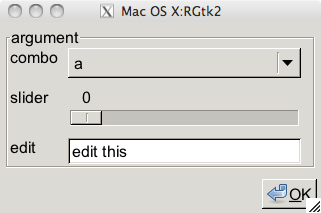
\includegraphics[width=0.45\textwidth]{ex-33-macosx-rgtk2} &
     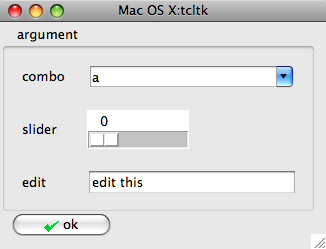
\includegraphics[width=0.45\textwidth]{fig-gWidgets-ex-33-tlctk}\\
     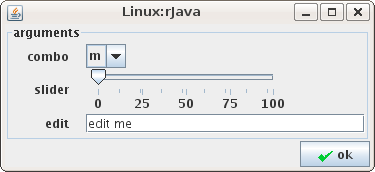
\includegraphics[width=0.45\textwidth]{ex-33-linux-rJava} &
     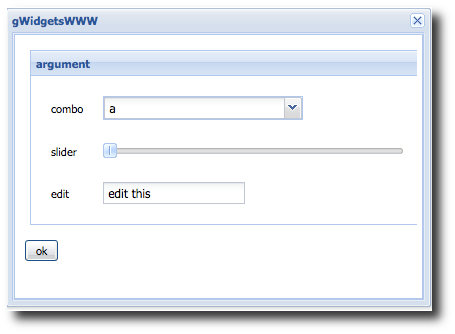
\includegraphics[width=0.45\textwidth]{ex-33-gWidgetsWWW}
 \end{tabular}
 \caption{The \pkg{gWidgets} package works with different operating systems and different GUI toolkits. This shows, the same code for \pkg{RGtk2}, \pkg{tcltk}, \pkg{rJava} and \pkg{gWidgetsWWW}. Note, each toolkit has it's own sizing ideas for the controls.}
  \label{fig:gWidgets-three-oses}
\end{figure}

% %% Make figure -- work on layout here
% \XXX{Do mac, windows}
% \begin{figure}
%   \centering
%   \begin{tabular}{lccc}
%     & \pkg{RGtk2} & \pkg{tcltk} & \pkg{rJava} 
%     \\
%     L &
%     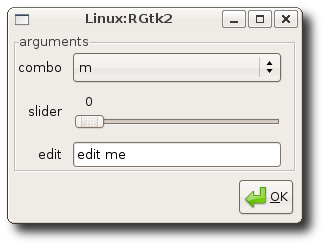
\includegraphics[width=0.3\textwidth]{ex-33-linux-rgtk2.png} &
%     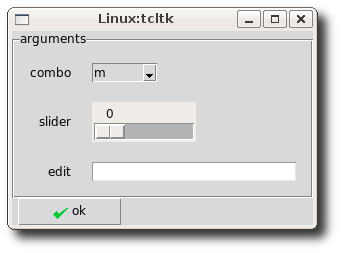
\includegraphics[width=0.3\textwidth]{ex-33-linux-tcltk} &
%     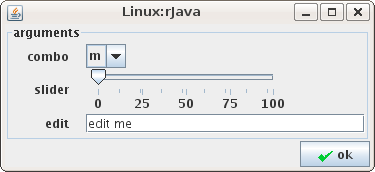
\includegraphics[width=0.3\textwidth]{ex-33-linux-rJava} 
%     \\
%     W &
%     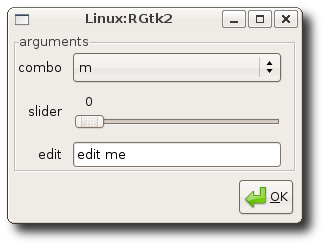
\includegraphics[width=0.3\textwidth]{ex-33-linux-rgtk2} &
%     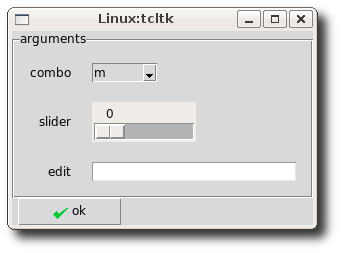
\includegraphics[width=0.3\textwidth]{ex-33-linux-tcltk} &
%     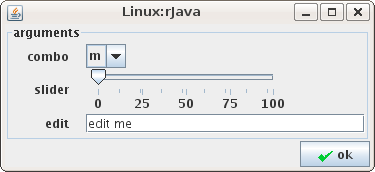
\includegraphics[width=0.3\textwidth]{ex-33-linux-rJava} 
%     \\
%     Mac &
%     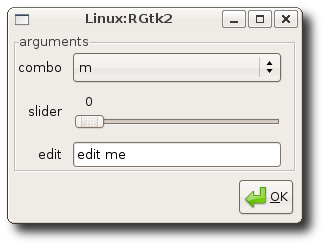
\includegraphics[width=0.3\textwidth]{ex-33-linux-rgtk2} &
%     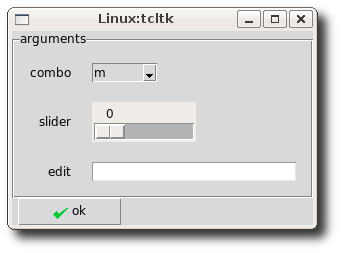
\includegraphics[width=0.3\textwidth]{ex-33-linux-tcltk} &
%     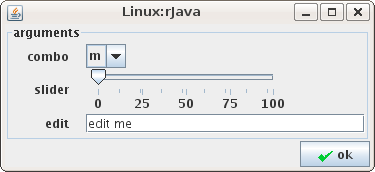
\includegraphics[width=0.3\textwidth]{ex-33-linux-rJava}
%   \end{tabular}
%   \caption{The \pkg{gWidgets} package works with different operating systems and different GUI toolkits. This shows the combination of \code{linux}, \code{Mac OS X (10.5)} and \code{Windows XP} and the packages \pkg{RGtk2}, \pkg{tcltk}, and \pkg{rJava}}
%   \label{fig:three-oses-three-toolkits}
% \end{figure}


% \begin{figure}
%   \centering
%   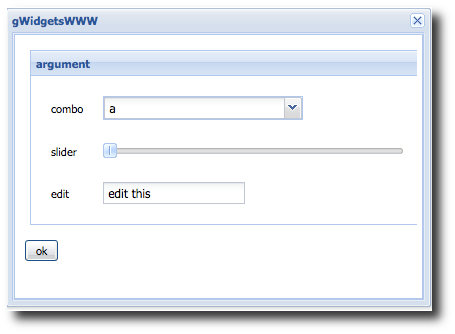
\includegraphics[width=.45\textwidth]{ex-33-gWidgetsWWW}
%   \caption{A GUI shown using \pkg{gWidgetsWWW}.}
%   \label{fig:gWidgetsWWW-same-gui}
% \end{figure}


\section{Startup}
%% starting package
The \pkg{gWidgets} package is loaded as other \R\/ packages:
\begin{Schunk}
\begin{Sinput}
 require(gWidgets)
\end{Sinput}
\end{Schunk}

A toolkit package is loaded when the first command is issued. If a
user does not have a toolkit installed, then a message indicating the
need to install an appropriate package is given.

%% Choice of toolkit
If a user has exactly one toolkit package installed, then that will be
used. But it is possible for more than one to be installed, in which
case the user is prompted to choose one through an interactive menu. This
choice can be avoided by setting the option \args{guiToolkit} to the
underlying \R\/ package name, as in
\begin{Schunk}
\begin{Sinput}
 options("guiToolkit"="RGtk2")
\end{Sinput}
\end{Schunk}
The value is the name of one of the \R\/ packages that \pkg{gWidgets} can
use.~\footnote{As of writing, this is either \pkg{RGtk2}, \pkg{tcltk}, or
\pkg{rJava}. The \pkg{gWidgetsWWW} package does not use \pkg{gWidgets}
for dispatch, rather it is loaded directly.}
Although in theory the different toolkits can be used together, in
practice the different eventloops created by each often lead to issues
that can lockup the \R\/ process.





\section{Constructors}
\label{sec:constructors}
%% constructors
GUI objects are produced by constructors. In
\pkg{gWidgets} most constructors have the following form: 
\begin{Schunk}
\begin{Sinput}
 gname(arguments, handler = NULL, action = NULL, 
       container = NULL,...,toolkit=guiToolkit())
\end{Sinput}
\end{Schunk}
where the \code{arguments} vary depending on the object being made. 

\subsection{Return value}

Not only do constructors create visible GUI objects they also return a
useful \R\/ object. Except for modal dialog constructors, this is an
S4 object of a certain class containing two components \code{toolkit}
and \code{widget}. The \code{toolkit} can be specified at time of
construction allowing tookits, in theory, to be mixed. Otherwise, the
\code{guiToolkit} funtion returns the currently selected toolkit, or
queries for one if none is selected point about dispatch
Constructors dispatch on the \code{toolkit} value to call the appropriate
constructor in the toolkit implementation. The return value from the
toolkit's constructor is kept in the \code{widget} component.  Generic
methods have a double dispatch when called. The first dispatch is
based on the \code{toolkit} value which calls a second generic
implemented in the toolkits with a different name (\code{svalue}
dispatches to \code{.svalue}). The tookit generic, then dispatches
based on the class of \code{widget} component and perhaps other
arguments given to the generic. The actual class of the S4 object
returned by the first constructor is (mostly) not considered, but when
we refer to methods for an object, we gloss over this double dispatch
and think of it as a single dispatch. This design allows the toolkit
packages the freedom to implement their own class structure. 

%% methods
As with most \R\/ objects, one calls generic functions to interact
programatically with the object. The \pkg{gWidgets} package
provides some familiar S3 methods, for the appropriate objects, for the
familiar generics \generic{[}, \generic{[$<$-}, \generic{dim},
\generic{length}, \generic{names}, \generic{names$<$-},
\generic{dimnames}, \generic{dimnames$<$-}, \generic{update}. In
addition, it provides new generics listed in
Table~\ref{tab:gWidgets-methods}. 

These new generics provide a means to query and set the primary value
of the widget (\meth{svalue}, \meth{svalue\ASSIGN}), and various methods
to effect the display of the widget (\meth{visible\ASSIGN},
\meth{font\ASSIGN}, \meth{enabled\ASSIGN}, \meth{focus\ASSIGN}). The
methods \meth{tag} and \meth{tag\ASSIGN} are implemented to bypass the
pass-by-copy issues that can make GUI programming awkward at times.


%% insufficiency of API
The \pkg{gWidgets} API provides just a handful of generic functions
for manipulating an object compared to the number of methods typically
provided by a GUI toolkit for a similar object. Although this
simplicity makes \pkg{gWidgets} easier to work with, one may wish to
get access to the underlying toolkit object to work at that level. The
\generic{getToolkitWidget} will provide that object. We don't
illustrate this, as we try to stay toolkit agnostic in our examples.


%% table of new methods
\begin{table}
\centering
\label{tab:gWidgets-methods}
\caption{Generic functions provided or used in \pkg{gWidgets} API.}
\begin{tabular}{@{}lp{0.6\textwidth}@{}}
\toprule

Method&Description\\
\midrule
\meth{svalue, svalue\ASSIGN}&Get or set value for widget\\\meth{[, [\ASSIGN}&Refers to values in data store\\\meth{length}&\meth{length} of data store\\\meth{dim}&\meth{dim} of data store\\\meth{names}&\meth{names} of data store \\\meth{dimnames}&\meth{dimnames} of data store\\\meth{update}&Update widget values\\\meth{size\ASSIGN}&Set size of widget in pixels\\\meth{show}&Show widget if not visible\\\meth{dispose}&Destroy widget or its parent\\\meth{isExtant}&Does \R\/ object refer to GUI object that still exists\\\meth{enabled, enabled\ASSIGN}&Adjust sensitivity to user input\\\meth{visible, visible\ASSIGN}&Adjust widget visibility.\\\meth{focus\ASSIGN}&Sets focus to widget\\\meth{defaultWidget\ASSIGN}&Set widget to have initial focus in a dialog\\\meth{insert}&Insert text into a multi-line text widget\\\meth{font\ASSIGN}&Set a widget's font\\\meth{tag, tag\ASSIGN}&Sets an attribute for a widget that persists through copies\\\meth{id, id\ASSIGN}&A unique ID for a widget\\\meth{getToolkitWidget}&Returns underlying toolkit widget for low-level use
\\ \bottomrule
\end{tabular}
\end{table}% \begin{table}
%   \centering
%   \begin{tabular}{l@{\quad}p{.75\textwidth}}
% %    \toprule
%     \meth{svalue, svalue\ASSIGN} & Get or set value for widget\\
%     \meth{[, [\ASSIGN} & If widget has a data store, refers to these values \\
%     \meth{length} & \meth{length} of data store\\
%     \meth{dim} & \meth{dim} of data store\\
%     \meth{names} & \meth{names} of data store \\
%     \meth{dimnames} & \meth{dimnames} of data store\\
%     \meth{update} & update widget values\\
%     \meth{size\ASSIGN}& set size of widget in pixels\\
%     \meth{show}& show widget if not visible\\
%     \meth{dispose} & destroy widget or its parent\\
%     \meth{isExtant} & Does \R\/ object refer to GUI object that still exists\\
%     \meth{enabled, enabled\ASSIGN} & An enabled widget can receive input from the user\\
%     \meth{visible, visible\ASSIGN} & Is widget visible.\\
%     \meth{focus\ASSIGN} & Sets focus to widget\\
%     \meth{defaultWidget, defaultWidget\ASSIGN} & Makes widget have initial
%     focus in a dialog\\
%     \meth{insert} & Used to insert text into a multi-line text widget\\
%     \meth{font\ASSIGN} & Set the font for a widget\\
%     \meth{tag, tag\ASSIGN} & Sets an attribute for a widget that persists
%     through copies\\
%     \meth{id, id\ASSIGN} & A unique ID for a widget\\
%     \meth{getToolkitWidget} & Returns underlying toolkit widget for
%     low-level use\\
%     \bottomrule
%   \end{tabular}
%   \caption{Table of generic functions with methods specified by the \pkg{gWidgets} API.}
%   \label{tab:gWidgets-methods}
% \end{table}

%% modal
A few constructors create modal dialogs. These do not return objects,
as when they are visible the \R\/ sesssion is unresponsive.
Consequently they have no methods defined for them.  Instead, these
constructors return values produced by the dialogs, which in turn can
be used as arguments to functions.

\subsubsection{The \code{container} argument}

%% container argument
The constructors produce two types of objects: containers
(Table~\ref{tab:gWidgets-container-constructors}) and components (the
basic controls in Table~\ref{tab:gWidgets-control-widgets} and the
compound widgets in Table \ref{tab:gWidgets-compound-widgets}).  A GUI
consists of a heiarchical nesting of containers which in turn contain
other containers or components. In a GUI, except for top-level windows
and modal dialogs, every component and container is the child of some
parent container. In \pkg{gWidgets} this parent is specified with the
\args{container} argument when an object is constructed. This argument
name can always be abbreviated \args{cont}. In the construction of a
widget in \pkg{gWidgets}, the \meth{add} method for the parent
container is called with the new object as an argument and the values
passed through the \args{...}  argument as arguments.  We remark that
not all the toolkits (e.g., \pkg{RGtk2}) require one to combine the
construction of an object with the specification of the parent
container. We don't illustrate this, as the resulting code is not cross-toolkit.


\subsection{The \code{handler} and \code{action} arguments}
\label{sec:callbacks}


%% callbacks
For all the toolkits, when the user initiates some event with the
mouse or keyboard, the underlying toolkit will emit some signal. The
toolkits allow callbacks to be called when these signals are emitted
allowing the GUI to be made interactive. In \pkg{gWidgets}, the
callbacks are functions with signature \code{(h,...)} where \code{h}
is a list that contains user data. Some toolkits pass information
through the \code{...} argument. As this is not portable across
toolkits, we do not use this here. In general, the \code{obj}
component of \code{h} contains the widget that the callback is
assigned to, and the component \code{action} contains user-specified
data passed through the \args{action} argument of the contructor or
the \meth{addHandlerXXX} method (the \code{XXX} may be one of several
values). For some classes, extra information is passed along, for
instance for the drop target generic, the component \code{dropdata}
contains a string holding the drag-and-drop information.


A callback for an event can be specified through the \args{handler}
argument of a constructor, or added at a later time through the
``\meth{addHandlerXXX}'' methods. The generic \meth{addHandlerChanged} can
be used to add a callback for the most reasonably defined event. In
many cases, more than one event is reasonable. For example, for single
line text widgets the \meth{addHandlerChanged} responds when the user
finishes editing, whereas \meth{addHandlerKeystroke} is called each
time the keyboard is used.  Table~\ref{tab:gWidgets-callback-methods}
shows a list of the these other methods.  If these few methods are
insufficient, and toolkit-portability is not of interest, then the
\meth{addHandler} generic can be used to specify a toolkit-specific
signal and a callback.  When a \meth{addHandlerXXX} method is used,
the return value is an ID. This ID can be used with the method
\meth{removeHandler} to remove the callback, or with the methods
\meth{blockHandler} and \meth{unblockHandler} to temporarily block a
handler from being called.


\section{Drag and Drop}
\label{sec:drag-drop}

%% drag and drop
Drag and drop support is implemented through three methods: one to set a widget a drag source, one to set a widget as a drop target, and one to call a handler when a drop event passes over a widget. The \generic{addDropSource} method needs a widget and a handler specified to call when a drag and drop event is initiated. This handler should return the value that will be passed to the drop target. The default value is the value returned by \code{svalue} method on the object. The \generic{addDropTarget} method is used to allow a widget to receive a dropped value and to specify a handler to call when a value is dropped. The \code{dropdata} component of the first-argument list, \code{h}, holds the drop data in the call to the handler. The \generic{addDropMotion} is used to call a handler for the event that a drag event passes over a widget.

Unfortunately, the drag and drop implememtions in the toolkits are not all the same. Some toolkits simply use the native drag and drop support, which can not be changed.

\begin{table}
\centering
\label{tab:gWidgets-callback-methods}
\caption{Generic functions to add callbacks in \pkg{gWidgets} API.}
\begin{tabular}{@{}lp{0.6\textwidth}@{}}
\toprule

Method&Description\\
\midrule
\meth{addHandlerChanged}&Refers to the signal that is bound towhen the \args{handler} argument is used by theconstructor. Interpretation varies from widget to widget.\\\meth{addHandlerClicked}&Sets handler for when widget is clicked with (left) mouse button. May return position of click through components \code{x} and \code{y} of the \code{h}-list. \\\meth{addHandlerDoubleclick}&Sets handler for when widget is double clicked\\\meth{addHandlerRightclick}&Sets handler for when widget is right clicked\\\meth{addHandlerKeystroke}&Sets handler for when key ispressed. The \code{key} component is set to this valueif possible.\\\meth{addHandlerFocus}&Sets handler for when widget gets focus\\\meth{addHandlerBlur}&Sets handler for when widget loses focus\\\meth{addHandlerExpose}&Sets handler for when widget is first drawn\\\meth{addHandlerDestroy}&Sets handler for when widget is destroyed\\\meth{addHandlerUnrealize}&Sets handler for when widget is undrawn on screen\\\meth{addHandlerMouseMotion}&Sets handler for when widget has mouse go over it\\\meth{addHandler}&For non cross-toolkit use, allows one to specify an underlying signal from the graphical toolkit\\\meth{removeHandler}&Remove a handler from a widget\\\meth{blockHandler}&Temporarily block a handler from being called\\\meth{unblockHandler}&Restore handler that has been blocked\\\meth{addHandlerIdle}&Call a handler during idle time\\\meth{addPopupmenu}&Bind popup menu to widget\\\meth{add3rdMousePopupmenu}&Bind popup menu to right mouse click\\\meth{addDropSource}&Specify a widget as a drop source\\\meth{addDropMotion}&Sets handler to be called when drag event mouses over the widget\\\meth{addDropTarget}&Sets handler to be called on a drop event. Adds the component \code{dropdata}.
\\ \bottomrule
\end{tabular}
\end{table}
% \begin{table}
%   \centering
%   \begin{tabular}{l@{\quad}p{.75\textwidth}}
% %    \toprule
%     \meth{addHandlerChanged} & Refers to the signal that is bound to
%     when the \args{handler} argument is used by the
%     constructor. Interpretation varies from widget to widget.\\
%     \meth{addHandlerClicked} & Sets handler for when widget is clicked with (left)
%     mouse button. May return position of click through components
%     \code{x} and \code{y} of the \code{h}-list. \\ 
%     \meth{addHandlerDoubleclick} &  Sets handler for when widget is
%     double clicked \\
%     \meth{addHandlerRightclick} & Sets handler for when widget is
%     right clicked\\
%     \meth{addHandlerKeystroke} & sets handler for when key is
%     pressed. The \code{key} component is set to this value if possible.\\
%     \meth{addHandlerFocus} & sets handler for when widget gets focus\\
%     \meth{addHandlerBlur} & sets handler for when widget loses focus\\
%     \meth{addHandlerExpose} & Sets handler for when widget is first drawn\\
%     \meth{addHandlerDestroy} & Sets handler for when widget is destroyed\\
%     \meth{addHandlerUnrealize} & Sets handler for when widget is
%     undrawn on screen\\
%     \meth{addHandlerMouseMotion} & Sets handler for when widget has
%     mouse go over it\\
%     \meth{addHandler} & To use underlying signal from graphical toolkit\\
%     \meth{removeHandler}& Remove a handler from a widget\\
%     \meth{blockHandler}& Temporarily block a handler from being called\\
%     \meth{unblockHandler}& Restore handler that has been blocked\\
%     \meth{addHandlerIdle} & Call a handler during idle time\\
%     \meth{addPopupmenu} & Bind popup menu to widget\\
%     \meth{add3rdMousePopupmenu} & Bind popup menu to right mouse click\\
%     \meth{addDropSource} & Specify a widget as a drop source\\
%     \meth{addDropMotion} & Sets handler to be called when drag event mouses over the widget\\
%     \meth{addDropTarget} & Sets handler to be called on a drop event. Adds the component \code{dropdata}.\\
%     \bottomrule
%   \end{tabular}
%   \caption{Table of generic functions for adding callbacks to \pkg{gWidgets} objects}
%   \label{tab:gWidgets-callback-methods}
% \end{table}



\chapter{\pkg{gWidgets}: Containers}
\label{sec:gWidgets-Containers}
%% Basic Containers


% \begin{table}
%   \centering
%   \begin{tabular}{l@{\quad}p{.75\textwidth}}
% %    \toprule
%     \constructor{gwindow} & Creates a top-level window\\
%     \constructor{ggroup} & Creates a box-like container\\
%     \constructor{gframe} & Creates a container with a text label \\
%     \constructor{gexpandgroup} & Creates a container with a label and
%     expand/collapse trigger\\ 
%     \constructor{gpanedgroup} & Creates a container for two child widgets
%     with a handle to assign allocation of space\\
%     \constructor{glayout} & A grid container\\
%     \constructor{gnotebook} & A tabbed notebook container for holding a
%     collection of child widgets\\
%     \bottomrule
%   \end{tabular}
%   \caption{Table of container constructors in \pkg{gWidgets}}
%   \label{tab:gWidgets-container-constructors}
% \end{table}

The \pkg{gWidgets} package provides a few useful containers: top-level
windows, box containers, grid-like containers and notebook containers.

\section{Top-level windows}
\label{sec:gWidgets-top-level-windows}

The \constructor{gwindow} constructor creates top-level windows. The
title of the window can be set during construction via the
\argument{title}{gwindow} argument or later through the
\meth{svalue\ASSIGN} method. As well, the initial size can be set
through the \argument{width}{gwindow} and \argument{height}{gwindow}
arguments. This initial size is the default size, but may be adjusted
later through the \method{size}{gwindow} method or through the window
manager. The \argument{visible}{gwindow} argument controls whether the
window is initially drawn. If not drawn initially, the
\method{visible\ASSIGN}{gwindow} method, taking a logical value, can be used draw the window
later in a program.  The default is to initially draw the window, but often it is good practice to suppress the initial drawing, especially for displaying GUIs with several controls as the
incremental  drawing of subsequent child components can make the
GUI seem sluggish.


Windows can be closed programatically with the
\method{dispose}{gwindow} method. Windows may also be closed through
the window manager, by clicking a close icon in the title bar.  The
\argument{handler}{gwindow} argument is called just before the window
is destroyed, but will not prevent that from happening.  The
\method{addHandlerUnrealize}{gwindow} method can be used to call a
handler between the initial click of the close icon and the subsequent
destroy event of the window. This handler must return a logical value:
if \code{TRUE} the window will not be destroyed, if \code{FALSE} the
window will be, as illustrated in the example.

The initial placement of a window will be decided by the window
manager, unlesss the \argument{parent}{gwindow} argument is
specified. If this is done with a vector of $x$ and $y$ pixel values,
the upper left corner will be placed there. If it is specified as a
\code{gwindow} instance, the new window will be positioned over the
specified window and be disposed of when the parent widget is. This is useful, say,
when a main window opens a dialog window to gather values.

In the document object model, the use of menubars, toolbars and
statusbars is often reserved for the main window, while dialogs are
not decorated so. In \pkg{gWidgets} it is suggested that these be
added only to a top-level window and required by some toolkits.

\begin{table}
\centering
\label{tab:gWidgets-container-constructors}
\caption{Constructors for container objects}
\begin{tabular}{@{}lp{0.6\textwidth}@{}}
\toprule

Constructor&Description\\
\midrule
\constructor{gwindow}&Creates a top-level window\\\constructor{ggroup}&Creates a box-like container\\\constructor{gframe}&Creates a container with a text label\\\constructor{gexpandgroup}&Creates a container with a label and trigger to expand/collapse\\\constructor{gpanedgroup}&Creates a container for two child widgets with a handle to assign allocation of space.\\\constructor{glayout}&A grid container\\\constructor{gnotebook}&A tabbed notebook container for holding a collection of child widgets
\\ \bottomrule
\end{tabular}
\end{table}

\begin{example}{An example of \constructor{gwindow}}{gWidgets-gwindow-ex}

  To illustrate, the following will open a new window. The initial
  drawing is postponed until after a button is placed in the window.
\begin{Schunk}
\begin{Sinput}
 w1 <- gwindow("parent window", visible=FALSE)
 b <- gbutton("a button", cont=w1)
 visible(w1) <- TRUE
\end{Sinput}
\end{Schunk}
This shows how one might use the \argument{parent}{gwindow} argument
to specify where a sub-window will be placed.
\begin{Schunk}
\begin{Sinput}
 w2 <- gwindow("child window", width=100, height=100, 
               parent=w1)               # center on w1
 b <- gbutton("button on child", cont = w2)
 dispose(w1)                           # closes w2 also
\end{Sinput}
\end{Schunk}


This shows how the \method{addHandlerUnrealize}{gwindow} method can be
used to intercept the closing of the window through the ``close'' icon
of the window manager. The \code{gconfirm} dialog returns \code{TRUE}
or \code{FALSE} depending on the button clicked, as will be explained
in \ref{sec:gWidgets-modal-dialogs}.
\begin{Schunk}
\begin{Sinput}
 w <- gwindow("Close through the window manager")
 id <- addHandlerUnrealize(w, handler=function(h,...) {
   !gconfirm("Really close", parent=h$obj)
 })
\end{Sinput}
\end{Schunk}
% Grid:
% RGtk2, tcltk
% mac <- c(TRUE,TRUE)
% linux <- c(TRUE, TRUE)
% windows <- c(TRUE,)
\end{example}

\begin{table}
\centering
\label{tab:gWidgets-container-methods}
\caption{Container methods}
\begin{tabular}{@{}lp{0.6\textwidth}@{}}
\toprule

Method&Description\\
\midrule
\meth{add}&Adds a child object to a parent container. Called when a parent container is specified to the \args{container} argument, in which case, the \args{...} arguments are passed to this method\\\meth{delete}&Remove a child object from a parent container
\\ \bottomrule
\end{tabular}
\end{table}

\section{Box containers}
\label{sec:gWidgets-box-containers}

The container produced by \constructor{gwindow} is intended to contain
just a single child widget, not several. This section demonstrates the
box containers produced by \constructor{ggroup} that can be used to
hold multiple child components. Through nesting, fairly complicated
layouts can be produced.

\subsection{The \code{ggroup} container}
\label{sec:gWidgets-ggroup-container}
  
The \constructor{ggroup} box container provides an argument
\argument{horizontal}{ggroup} to specify whether the child widgets
are packed in horizontally left to right (the default) or vertically
from top to bottom. Unlike with the underlying graphical toolkits,
there is no means to specify other styles of packing such as from the
ends, or in the middle by some index.

\paragraph{add}
When packing in child widgets, the \method{add}{ggroup} method is
used. In our examples, this is called internally by the constructors
when the \args{container} argument is specified. The appropriate
\args{...}  values for a constructor are passed to the \meth{add}
method. For \constructor{ggroup} the important ones are \args{expand}
and \args{anchor}. When more space is allocated to a child, then is
needed by that child, the \args{expand=TRUE} argument will cause the
child to grow to fill the available space in both directions. (No
means is available in \pkg{gWidgets} to restrict to just one
direction.) If \args{expand=TRUE} is not specified, then the
\args{anchor} argument will instruct how to anchor the child into the
space allocated. The direction is specified by $x$-$y$ coordinates
with both values from either $-1$, 0 or $1$, where 1 indicates top and
right, whereas $-1$ is left and bottom. The example will demonstrate
their use.

\paragraph{delete}
The \method{delete}{ggroup} method can be used to remove a child component from a box container. In some toolkits, this child may be added back at a later time, but this isn't part of the API.

\paragraph{Spacing and sizing}
For spacing between the child components, the argument
\argument{spacing}{ggroup} may be used to specify, in pixels, the
amount of space between the child widgets. This can later be set
through the \method{svalue}{ggroup} method. The method
\method{addSpace}{ggroup} can add space between two widgets packed
next to each other, whereas the method \method{addSpring}{ggroup} will place
an invisible spring between two widgets, forcing them apart.  Both are
useful for laying out buttons.

The overall size of \code{ggroup} container is controlled through it
being a child of its parent container. However, a size can be assigned
through the \method{size\ASSIGN}{ggroup} method. This will be a
preferred size, but need not be the actual size, as the container may
need to be drawn larger to accomodate its children. The argument
\argument{use.scrollwindow}{ggroup} when specified as \code{TRUE} will
add scrollbars to the box container so that a fixed size can be
maintained. Although, it is generally considered a poor idea to use
scrollbars when there is a chance the key controls for a dialog will
be hidden.

%%\XXX{not inspiring}

\begin{example}{Example of \constructor{ggroup} usage}{gWidgets-ggroup-ex}

This example shows the nesting of vertical and horizontal box containers and
the effect of the \code{expand} and \code{anchor}
arguments. Figure~\ref{fig:ggroup-example} shows how it is implemented
in two different toolkits.
\begin{figure}
  \centering
  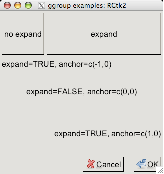
\includegraphics[width=.45\textwidth]{ex-gWidgets-ggroup-RGtk2}\quad
  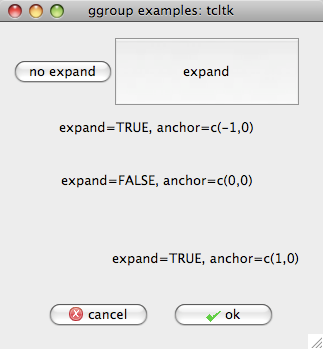
\includegraphics[width=.45\textwidth]{ex-gWidgets-ggroup-tcltk}
 \caption{Use of \code{expand}, \code{anchor}, \code{addSpace} and
     \code{addSpring} with the \code{ggroup} constructor in \pkg{gWidgetsRGtk2} and \pkg{gWidgetstcltk}}
  \label{fig:ggroup-example}
\end{figure}





\begin{Schunk}
\begin{Sinput}
 w  <- gwindow("ggroup examples")
 g  <- ggroup(cont=w, horizontal=FALSE, expand=TRUE)
 g1 <- ggroup(cont=g, expand=TRUE)
 b  <- gbutton("no expand", cont=g1)
 b  <- gbutton("expand", cont=g1, expand=TRUE)
 g2 <- ggroup(cont=g)
 l  <- glabel("expand=TRUE, anchor=c(-1,0)", anchor=c(-1,0), 
             expand=TRUE, cont=g2)
 g3 <- ggroup(cont=g, expand=TRUE)
 l  <- glabel("expand=FALSE, anchor=c(0,0)", anchor=c(0,0), 
             expand=TRUE, cont=g3)
 g4 <- ggroup(cont=g, expand=TRUE)
 l  <- glabel("expand=TRUE, anchor=c(1,0)", anchor=c(1,0), 
             expand=TRUE, cont=g4)
\end{Sinput}
\end{Schunk}
  
This demonstrates how one might use the \meth{addSpace} and \meth{addSpring}
methods in a button bar.
\begin{Schunk}
\begin{Sinput}
 g5 <- ggroup(cont=g, expand=FALSE)
 addSpring(g5)
 b  <- gbutton("cancel", cont=g5, handler=function(h,..) dispose(w))
 addSpace(g5, 10)
 b  <- gbutton("ok", cont=g5)
\end{Sinput}
\end{Schunk}
\end{example}

The next example shows an alternative to the expand group widget.

\begin{example}{The \meth{delete} method of \code{ggroup}}{ex-gWidgets-ggroup-delete}
This example shows nested ggroup containers and the use of the
\method{delete}{ggroup} method to remove a child widget from a
container. In this application, a box is set aside at the top of the
window to hold a message that can be set via \code{openAlert} and
closed with \code{closeAlert}. This example works better under
\pkg{RGtk2}, as the space allocated to the alert is reclaimed when
it is closed.


This code sets up the area for the alert box to appear from.
\begin{Schunk}
\begin{Sinput}
 w <- gwindow("Alert box example")
 g <- ggroup(horizontal=FALSE, cont = w)
 alertBox <- ggroup(cont = g)
 mainBox <- ggroup(cont = g, expand=TRUE)
 l <- glabel("main box label", cont = mainBox, expand=TRUE)
 ig <- NULL                              # global
\end{Sinput}
\end{Schunk}

These two functions will open and close the alert box respectively. In
this example we use the global value, \code{ig}, to store the inner group.
\begin{Schunk}
\begin{Sinput}
 openAlert <- function(message="message goes here") {
   ig <<- ggroup(cont=alertBox)
   glabel(message, cont = ig)
 }
 closeAlert <- function() delete(alertBox, ig)
\end{Sinput}
\end{Schunk}

The state of the box can be toggled programattically via
\begin{Schunk}
\begin{Sinput}
 QT <- openAlert("new message")                # open
 QT <- closeAlert()                            # close
\end{Sinput}
\end{Schunk}

\end{example}


\subsection{The \code{gframe} and \code{gexpandgroup} containers}
\label{sec:gWidgets-decorated-cont}

Framed containers are used to set off elements and are provided by
\constructor{gframe}. Expandable containers are used to preserve
screen space unless requested and are provided by
\constructor{gexpandgroup}. Both of these containers can be used in
place of the \constructor{ggroup} container.

In addition to the \code{ggroup} arguments, the \constructor{gframe}
constructor has the arguments \argument{text}{gframe} to specify the
text marking the frame and \argument{pos}{gframe} to specify the
positioning of the text, using 0 for left and 1 for right. If the
toolkit supports markup, such as \pkg{RGtk2}, the
\argument{markup}{gframe} argument takes a logical indicating if
markup is being used in the specification of \args{text}.  The
\method{names}{gframe} method can be used to get and set the label
after construction of the widget.


The \constructor{gexpandgroup} constructor, like \code{gframe}, has
the \code{text} argument, but no \code{pos} argument for positioning
the text label. The widget has two states, which may be toggled either
by clicking the trigger or through the
\method{visible\ASSIGN}{gexpandgroup} method.  A value of \code{TRUE}
means the child is visible. The
\method{addHandlerChanged}{gexpandgroup} method is used to specify a
callback for when the widget is expanded.

\begin{example}{The \constructor{gframe} and \constructor{gexpandgroup} containers}{gWidgets-gframe-gexpandgroup-ex}
This example shows how the \constructor{gframe} container can be used.
\begin{Schunk}
\begin{Sinput}
 w <- gwindow("gframe example")
 f <- gframe(text="title", pos=1, cont=w)
 l <- glabel("Some text goes here", cont=f)
 names(f) <- "new title"
\end{Sinput}
\end{Schunk}

This is a similar example for \constructor{gexpandgroup}.
\begin{Schunk}
\begin{Sinput}
 w <- gwindow("gexpandgroup example")
 g <- gexpandgroup(text="title", cont=w)
 l <- glabel("Some text goes here", expand=TRUE, cont=g)
 visible(g) <- FALSE
 visible(g) <- TRUE                      # toggle visibility
\end{Sinput}
\end{Schunk}
\end{example}




\section{Paned containers: the \code{gpandedgroup} container}
\label{sec:gWidgets-gpanedgroup-container}

The \constructor{gpanedgroup} constructor produces a container which
has two children. The children are aligned side-by-side by default, or
top to bottom if the \argument{horizontal}{gpanedgroup} argument is given as \code{FALSE}. These two
children are separated by a visual gutter which can be adjusted using
the mouse to allocate the space between the two children. This can
also be done programatically using the \method{svalue\ASSIGN}{gpanedgroup}
method where  a value from 0 to 1 specifies the proportion of space allocated to the leftmost (topmost) child.

To add children, the container should be used as the parent container
for two constructors. These can be other container constructors which
is the typical usage for more complicated layouts.
(For toolkits which support the separation of widget
construction and layout, the \constructor{gpanedgroup} constructor can
have two children specified to the arguments
\argument{widget1}{gpanedgroup} and \argument{widget2}{gpanedgroup}.)

\begin{example}{Paned groups}{ex-gWidgets-panedgroups}
  This example shows how one could use this container.
\begin{Schunk}
\begin{Sinput}
 w <- gwindow("gpanedgroup example", visible=FALSE)
 pg <- gpanedgroup(cont=w)
 g <- ggroup(cont=pg)                  # left child
 l <- glabel("left child", cont=g)
 b <- gbutton("right child", cont=pg)
 visible(w) <- TRUE
\end{Sinput}
\end{Schunk}
To adjust the sash position, one can do:
\begin{Schunk}
\begin{Sinput}
 svalue(pg) <- .5
\end{Sinput}
\end{Schunk}
\end{example}


  
\section{Tabbed notebooks: the \code{gnotebook} container}
\label{sec:gWidgets-gnotebook}

The \constructor{gnotebook} constructor produces a tabbed notebook
container. The constructor has the argument \argument{tab.pos}{gnotebook}
to specify the location of the tabs. A value of 1 through 4 with 1
being botton, 2 left side, 3 top and 4 right side being used, with the
default being 3. (Not available for all toolkits.) The \argument{closebuttons}{gnotebook} argument takes a logical
indicating whether the tabs should have close buttons on them. In this
case, the argument \argument{dontCloseThese}{gnotebook} can be used to
specify which tabs, by index, should not be closable. (Some toolkits do
not implement these features though.)

The \method{add}{gnotebook} method for the notebook container uses the \argument{label}{add}
argument to specify the tab label. As this is called implicitly when a a widget is constructed, this argument is specified to the constructor.

\paragraph{Methods}
The \method{svalue}{gnotebook} method returns the index of the
currently raised tab, whereas \method{svalue\ASSIGN}{gnotebook} can be
used to switch the page to the specified tab. The currently shown tab can be
removed using the \method{dispose}{gnotebook} method. To remove a
different tab, use this method in combination with
\meth{svalue\ASSIGN}. When removing many tabs, you may want to start
from the end as otherwise the tab positions change, which can be
confusing when using a loop. The \method{names}{gnotebook} method can
be used to retrieve the tab names, and
\method{names\ASSIGN}{gnotebook} to set the names. The
\method{length}{gnotebook} method returns the number of pages held by
the notebook.


\begin{example}{Tabbed notebook example}{ex-gWidgets-gnotebook}
  A simple example follows. The \args{label} argument is passed along from the constructor
  to the \meth{add} method for the notebook instance.
\begin{Schunk}
\begin{Sinput}
 w <- gwindow("gnotebook example")
 nb <- gnotebook(cont=w, tab.pos=3)
 l <- glabel("first page", cont=nb, label="one")
 b <- gbutton("second page", cont=nb, label="two")
\end{Sinput}
\end{Schunk}
To set the page to the first one:
\begin{Schunk}
\begin{Sinput}
 svalue(nb) <- 1
\end{Sinput}
\end{Schunk}
To remove the first page (the current one)
\begin{Schunk}
\begin{Sinput}
 dispose(nb)
\end{Sinput}
\end{Schunk}
\end{example}

\section{Grid layout: the \code{glayout} container}
\label{sec:gWidgets-glayout-container}

The layout of dialogs and forms is usually seen with some form of
alignment between the widgets. The \constructor{glayout} constructor
provides a grid container to do so, using matrix notation to specify location of the children.
The argument
\argument{homogeneous}{glayout} can be used to specify that each cell
take up the same size, the default is \code{FALSE}. Spacing between each cell may be specified through the \argument{spacing}{glayout} argument.

Children may be added to the grid at a specific row and column, and a
child may span more than one row or column. To specify this, \R's
matrix notation, \code{[\ASSIGN}, is used with the indices indicating
the row and column.  When a child is to span more than one row or
column, the corresponding index should be a vector of indices
indicating so.  There is no \code{[} method defined to return the
child components.  
To add a child, the \code{glayout} container should be specfied as the \code{container} and be on the left hand side of the \code{[\ASSIGN} call. For convenience, if the right hand side is a string, a label will be generated.
To align a widget within a cell, the
\argument{anchor}{add} argument of the \code{[\ASSIGN}{glayout} method
is used. The example illustrates how this can be used to achieve a center balance.


\begin{example}{Layout with \constructor{glayout}}{ex-gWidgets-glayout}
  This example shows how a simple form can be given an attractive
  layout using a grid container. It uses the \constructor{gedit}
  constructor to provide a single-line text entry widget. As the
  matrix notation does not have a means to return the child widget (a
  \code{[} method say), we store the values of the
  \constructor{gedit} widgets into variables.
\begin{Schunk}
\begin{Sinput}
 w <- gwindow("glayout example")
 tbl <- glayout(cont=w)
 right <- c(1,0); left <- c(-1,0)
 tbl[1,1, anchor=right] <- "name"
 tbl[1,2, anchor=left ] <- (name <- gedit("", cont=tbl))
 tbl[2,1, anchor=right] <- "rank"
 tbl[2,2, anchor=left ] <- (rank <- gedit("", cont=tbl))
 tbl[3,1, anchor=right] <- "serial number"
 tbl[3,2, anchor=left ] <- (snumber <- gedit("", cont=tbl))
\end{Sinput}
\end{Schunk}
\end{example}







\chapter{\pkg{gWidgets}: Control Widgets}
\section{Basic controls}
\label{sec:gWidgets-controls}
%% orgainze by function

\XXX{Where to integrate methods such as enabled?}
\XXX{stock icons}
\XXX{addHandler text -- done here with first, but could be elsewhere}
\XXX{drag and drop example}
  

  
This section discusses the basic controls provided by
\pkg{gWidgets}.

\begin{table}
\centering
\label{tab:gWidgets-control-widgets}
\caption{Table of constructors for control widgets in \pkg{gWidgets}. Most, but not all, are implemented for each toolkit.}
\begin{tabular}{@{}lp{0.7\textwidth}@{}}
\toprule

Constructor&Description\\
\midrule
\constructor{glabel}&A text label\\\constructor{gbutton}&A button to initiate an action \\\constructor{gradio}&A radio button group\\\constructor{gcheckbox}&A checkbox\\\constructor{gcheckboxgroup}&A group of checkboxes\\\constructor{gcombobox}&A drop-down list of values\\\constructor{gtable}&A table (vector or data frame) of values for selection\\\constructor{gslider}&A slider to select a value\\\constructor{gspinbutton}&A spinbutton to select from a set of values\\\constructor{gedit}&Single line of editable text\\\constructor{gtext}&Multi-line text edit area\\\constructor{ghtml}&Display text marked up with HTML\\\constructor{gdf}&Data frame viewer and editor\\\constructor{gtree}&A display for heirarchical data\\\constructor{gimage}&A display for icons and images\\\constructor{ggraphics}&A widget containing a graphics device\\\constructor{gfilebrowser}&A widget to select a file or directory\\\constructor{gcalendar}&A widget to select a date\\\constructor{gaction}&A resusable definition of an action\\\constructor{gmenubar}&Puts a menubar on a top-level window \\\constructor{gtoolbar}&Adds a toolbar to a top-level window\\\constructor{gstatusbar}&Adds a status bar to a top-level window\\\constructor{gtooltip}&Add tooltip to widget\\\constructor{gseparator}&A widget to display a horizontal or vertical line
\\ \bottomrule
\end{tabular}
\end{table}%% place these as approporiate
% \begin{table}
%   \centering
%   \begin{tabular}{l@{\quad}p{.75\textwidth}}
% %    \toprule
%     \constructor{glabel} & A text label\\
%     \constructor{gbutton} & A button to initiate an action \\
%     \constructor{gcheckbox} & A checkbox widget\\
%     \constructor{gradio} & Constructs a radio button group\\
%     \constructor{gcheckboxgroup} & Constructs a group of checkboxes\\
%     \constructor{gcombobox} & Constructs drop down list of values\\
%     \constructor{gtable} & Shows a table (vector or data frame) of
%     values for selection\\ 
%     \constructor{gslider} & A slider to select a value\\
%     \constructor{gspinbutton} & A spinbutton to select from a set of values\\
%     \constructor{gedit} & One line of editable text\\
%     \constructor{gtext} & multi-line text edit\\
%     \constructor{ghtml} & Display text marked up with HTML\\
%     \constructor{gdf} & Data frame viewer and editor\\
%     \constructor{gtree} & Displays heirarchical data\\
%     \constructor{gimage} & Displays icons and images\\
%     \constructor{ggraphics} & A widget containing a graphics device\\
%     \constructor{gfilebrowser} & A widget to select a file or directory\\
%     \constructor{gcalendar} & A widget to select a date\\
%     \constructor{gaction} & a resusable definition of an action\\
%     \constructor{gmenubar} & Puts a menubar on a top-level window\\    
%     \constructor{gtoolbar} & Adds a toolbar to a top-level window\\
%     \constructor{gstatusbar} & Adds a status bar to a top-level window\\
%     \constructor{gseparator} & A widget to display a horizontal or vertical line\\
%     \bottomrule
%   \end{tabular}
%   \caption{Table of basic control constructors in \pkg{gWidgets}}
%   \label{tab:gWidgets-control-widgets}  
% \end{table}


\subsection{Buttons, Menubars, Toolbars}
\label{sec:gWidgets-buttons}

The button widget allows a user to initiate an action through clicking on
it. Buttons have labels -- usually verbs indicating action -- and often
icons. The \constructor{gbutton} constructor has an argument
\argument{text}{gbutton} to specify the text.  For text that matches
the stock icons, an icon will also be rendered. A list of stock icons is returned by \code{getStockIcons}. In common with the other controls, the argument
\argument{handler}{gbutton} is used to specify a callback and the
\argument{action}{gbutton} argument will be passed along to this
callback (unless it is a \code{gaction} object, whose case is described
below).

The click handler can be specified at construction, or afterward
through the \method{addHandlerClicked}{gbutton} which is also aliased
to the generic \method{addHandlerChanged}{gbutton}. 


%% Default
A new button may or may not have the focus when a GUI is
constructed. If it does have the focus, then the \kbd{return} key will
initiate the button click signal. To make a GUI start with its focus
on a button, the \method{defaultWidget}{gWidgets} method is available. 

%% methods
The \method{svalue}{gbutton} method will return button's label. The
method \method{svalue\ASSIGN}{gbutton} is used to set the label text.
Most GUIs will make a button insensitive to user input if the button's
action is not currently permissible. Toolkits draw such buttons in a
greyed out state. The \method{enabled\ASSIGN}{gWidgets} method can set or
disable whether a widget can accept input.


% As an example of the limitations of \pkg{gWidgets} compared to the
% underlying toolkits, within \pkg{gWidgets} there are no methods to set
% an icon, or add an mnemonic to the button.


\begin{example}{Hello world button}{ex-gWidgets-hello-world-button}
  This example shows how a button is assigned a handler to respond to
  click events.~\footnote{Each toolkit has its idiosyncracies. If this
    example is run using \pkg{RGtk2} the button will stretch to fill
    the space. At times this is not desired. Placing the button within
    a \code{ggroup} container can prevent this. Whereas, under
    \code{tcltk} the parent window will shrink to fit the button. The
    \meth{size} method can prevent this if it is not desired.} When
  working with handlers, one can use an object name that will be found
  through \R's scoping rules, or the components passed through the
  \code{h} argument, as below.

\begin{Schunk}
\begin{Sinput}
 w <- gwindow("Button example")
 b <- gbutton("Click me", cont=w)
 id <- addHandlerChanged(b, action=w, handler=function(h,...) {
   btnText <- svalue(h$obj)                   # or svalue(b)
   svalue(h$obj) <- paste("don't", btnText, "again") # set text
   enabled(h$obj) <- FALSE
   svalue(h$action) <- "Button example is finished" # set title
 })
\end{Sinput}
\end{Schunk}

\end{example}





\subsection{Actions}
\label{sec:gWidgets-actions}

In GUI programming an action is a reusable code object that can be
shared among buttons, toolbars, and menubars. Common to these three
controls are that the user expects some ``action'' to occur when a
value is selected. For example, some save dialog is summoned, or some
page is printed.
%%In the command framework, actions initiate commands.
Actions contain enough information to be displayed in several
manners. An action would contain some text, an icon, perhaps some
keyboard accelerator, and some handler to call when the action is
selected. When a particular action is not possible due to the state of
the GUI, it should be disabled, so as not to be sensitive to user interaction.

Actions in \pkg{gWidgets} are created through the
\constructor{gaction} contstructor. The arguments are
\argument{label}{gaction}, \argument{tooltip}{gaction},
\argument{icon}{gaction}, \argument{key.accel}{gaction} and the
standard \argument{handler}{gaction} and
\argument{action}{gaction}. The label appears as the text on a button,
the menu item or toolbar text, whereas the icon will decorate the same
if possible. For some toolkits, the tooltip pops up when the mouse hovers, as may be done
through the \code{tooltip<-} method for \pkg{gWidgets} objects.

\paragraph{methods}
The main methods for actions are \method{svalue\ASSIGN}{gaction} to
set the label text and \method{enabled\ASSIGN}{gaction} to adjust
whether the widget is sensitive to user input. All instances of the
action are set through one call. In some toolkits, such as
\pkg{RGtk2}, actions are bundled together into action groups. This
allows one to easy set the sensitivity of related actions at once. In
\R, one can store like actions in a list, and get similar
functionality by using \code{sapply}.

\paragraph{buttons}
An action can be assigned to a button by setting it as the
\argument{action}{gbutton} argument of the \code{gbutton} constructor, in which
case all other arguments for the constructor are ignored. 

Otherwise, actions are used as list components which define the
toolbar or menubar, as described in the following.



\subsection{Toolbars}
\label{sec:gWidgets-toolbars}

The document object model, when employed, often relies on the custom
that the main window showing the document possibly has a menu bar, a
toolbar and a status bar. Subwindows, such as those for dialogs, would
not have these decorations to emphasize their role in the GUI.


In \pkg{gWidgets}, toolbars (and menubars) are specified ahead of time as as a named
list. This is similar to how \pkg{RGtk2} can use an XML specification
to define a user interface, but unlike how menubars and toolbars can
be created one item at a time in the toolkits.

For a toolbar, the list has a simple structure. The list has named
components each of which either describes a toolbar item or a
separator. The toolbar items are specified by \code{gaction} instances
and separators by \code{gseparator} instances with no container
specified. (Alternatively, these items can be specified through lists as
described in the manual page.)


The \constructor{gtoolbar} constructor takes as its first argument the
list.  As toolbars belong to the window, the corresponding
\pkg{gWigdets} objects use a \constructor{gwindow} object as the
parent container. (Some of the toolkits relax this.)  The argument
\argument{style}{gtoolbar} can be one of \code{"both"},
\code{"icons"}, \code{"text"}, or \code{"both-horiz"} to specify how
the toolbar is rendered. Toolbars in \pkg{gWidgetstcltk} are not
native widgets, so the implementation uses aligned buttons.




\subsection{Menubars, popup menus}
\label{sec:gWidgets-menubars}

Menubars and popup menus are specified in a similar manner as toolbars with menu items
being defined through \code{gaction} instances, and visual separators
by \code{gseparator} instances. Menus differ from toolbars, as
sub-menus give a nested structure. This structure is specified using a
nested list as the component to describe the sub menu. The lists all
have named components, in this case the corresponding name is used to
label the sub menu item. For menu bars, it is typical that all the
top-level components be lists, but for popup menus, this wouldn't
necessarily be the case.

The main constructor \constructor{gmenu} has its first arugment to
specify the list, and the \code{container} argument to specify the
top-level window. 

In Mac OS X, toolbars may be drawn along the top of the screen, as is the custom of that OS.

\paragraph{Methods}
The main methods for toolbar and menubar instances are
the \method{svalue}{gmenu} method which will return the list. Whereas, the
\method{svalue\ASSIGN}{gmenu} method can be used to redefine the
menubar or toolbar. Use the \method{add}{gmenu} method to append to an
existing menubar or toolbar, again using a list to specify the new items.


\begin{example}{Menubar and toolbar example}{ex-gWidgets-menu-tool-status-bars}

The following commands create some standard looking actions. The
handler \code{f} is just a stub to be replaced in a real application.
\begin{Schunk}
\begin{Sinput}
 f <- function(...) print("stub")        # a stub
 aOpen <- gaction("open", icon="open", handler = f)
 aQuit <- gaction("quit", icon="quit", handler = f)
 aUndo <- gaction("undo", icon="undo", handler = f)
\end{Sinput}
\end{Schunk}

A menubar and toolbar are specified through a  named list, as is
illustrated next. The menubar list, has a nested list specifying a submenu.
\begin{Schunk}
\begin{Sinput}
 tl <- list(open = aOpen, quit = aQuit)
 ml <- list(File = list(
              open = aOpen, 
              sep = gseparator(), 
              quit = aQuit),
            Edit = list(
              undo = aUndo
              ))
\end{Sinput}
\end{Schunk}


Menubars and toolbars are added to top-level windows, so their parent
containers should be \code{gwindow} objects.
\begin{Schunk}
\begin{Sinput}
 w <- gwindow("Example of menubars, toolbars")
 mb <- gmenu(ml, cont=w)
 tb <- gtoolbar(tl, cont=w)
 l <- glabel("Test of DOM widgets", cont=w)
\end{Sinput}
\end{Schunk}


By disabling a \code{gaction} instance, we change the sensitivity of
all its realizations. Here this will only affect the menu bar.

\begin{Schunk}
\begin{Sinput}
 enabled(aUndo) <- FALSE
\end{Sinput}
\end{Schunk}

An ``undo'' menubar item, often changes its label when a new command
is performed, or the previous command is undone. The
\method{svalue\ASSIGN}{gaction} method can set the label text. This
shows how a new command can be added and how the menu item can be made
sensitive to mouse events.
\begin{Schunk}
\begin{Sinput}
 svalue(aUndo) <- "undo: command"
 enabled(aUndo) <- TRUE
\end{Sinput}
\end{Schunk}

%%\XXX{Citation needed}

Good GUI building principles suggest that one should not replace
values in the a menu, rather one should simply disable those that are
not being used. This allows the user to more easily become familiar
with the possible menu items. However, it may be useful to add to a
menu or toolbar. The \method{add}{gmenu} method can do so. For
example, to add a help menu item to our example one could do:
\begin{Schunk}
\begin{Sinput}
 hl <- list(help = list(
              help = gaction("manual", handler=f)
              ))
 add(mb, hl)
\end{Sinput}
\end{Schunk}




        
\end{example}

\paragraph{Popup menus}

Popup menus can be created for a right click event through the \constructor{add3rdMousePopupmenu} constructor. (Or \kbd{control-button-1} for Mac OS X.) This constructor has arguments \code{obj} to specify a widget, like a button, to initiate the popup, \argument{menulist}{gmenu} to specify the menu and optionally an \argument{action}{gmenu} argument.


\begin{example}{Popup menus}{ex-gWidgets-context-menus}
\begin{Schunk}
\begin{Sinput}
 w <- gwindow("Popup example")
 b <- gbutton("click me or right click me", cont=w, 
              handler=function(h, ...) {
                cat("You clicked me\n")
              })
 f <- function(h,...) cat("you right clicked on", h$action, "\n")
 mbList <- list(one = gaction("one", action="one", handler=f),
                two = gaction("two", action="two", handler=f)
                )
 add3rdMousePopupmenu(b, mbList)
\end{Sinput}
\end{Schunk}

\end{example}


\section{Text widgets}
\label{sec:text-widgets}

A number of widgets are geared toward the display or entry of
text. The \pkg{gWidgets} API defines \constructor{glabel} for
displaying a single-or multiple-line string of static text,
\constructor{gstatusbar} to place message labels at the foot of a
window, \constructor{gedit} for a single line of editable text, and
\constructor{gtext} for multi-line, editable text. For some toolkits,
a \constructor{ghtml} widget is also defined, but neither \code{RGtk2}
or \code{tcltk} have this implemented.

\subsection{Labels}
\label{sec:gWidgets-static-text}

The \constructor{glabel} constructor produces a basic label
widget. The label's text is specified through the
\argument{text}{glabel} argument. This is a character vector of length
1 or is coerced into one by collapsing the vector with newlines. The
\method{svalue}{glabel} method will return the text as a single
string, and the \method{svalue\ASSIGN}{glabel} method can be used to
set the text programatically. The \method{font\ASSIGN}{glabel} method
can also be used to set the text markup
(Table~\ref{tab:gWidgets-font-properties}).  For some toolkits, the
argument \argument{markup}{glabel} for the constructor takes a logical
value indicating if the text is in the native markup language (PANGO
for \code{RGtk2}).


The widget constructor also has the argument
\argument{editable}{glabel}, which when specified as \code{TRUE} will
add a handler to the event that the label is clicked that allows the
text to be edited. 
Although this is popular in some GUIs, say the tab
in a spreadsheet, it has not proven to be intuitive to most users, as
typically labels are not expected to change. In the wxWidgets toolkit labels are
constructed by a function named \code{staticText} to emphasize this
permanence.


\subsection{Statusbars}
\label{sec:gWidgets-statusbars}

Statusbars are simply labels placed at the bottom of a window to leave
informative, but non-disruptive, messages for the user.  The
\constructor{gstatusbar} constructor provides this widget.  The argument
\argument{text}{gstatusbar} can be given to set the intial text away
from its default of no message. Subsequent changes are made through
the \method{svalue\ASSIGN}{gstatusbar} method. As with toolbars and
menubars, a top-level window should be specified for the
\argument{container}{gstatusbar} argument.



\subsection{Single-line, editable text}
\label{sec:gWidgets-single-line-editable}

The \constructor{gedit} constructor produces a widget to display a
single line of editable text. The initial text can be set through the
\argument{text}{gedit} argument. 
If it is desirable to set the width of the widget, the
\argument{width}{gedit} argument allows the specification in terms of
number of characters allowed to display without horizontal scrolling. The width
of the widget may also be specified in pixel size through the
\method{size}{gWidgets} method.


\paragraph{Methods}
The text is returned by the
\method{svalue}{gedit} method and may be set through the
\method{svalue\ASSIGN}{gedit} method.
The \meth{svalue} method will return a character vector by
default. However, it may be desirable to use this widget to collect
numeric values or perhaps some other type of variable. One could write
code to coerce the character to the desired type, but it is sometimes
convenient to have the return value be a certain non-character
type. In this case, the \argument{coerce.with}{gedit} argument can be
used to specify a function of a single argument to call before the
value is returned by \meth{svalue}.

Some toolkits allow type-ahead values to be set. These values
anticipate what a user wishes to type and offers a means to complete a
word. The \method{[\ASSIGN}{gedit} method allows these values to be
specifed through a character vector, as in \code{obj[] \ASSIGN\/ values}.



\paragraph{Handlers}
The default handler for the \constructor{gedit} widget is called when
the text area is ``activated'' through it losing focus or the
\kbd{return} key being pressed. The
\method{addHandlerKeystroke}{gedit} method can assign a handler to be
called when a key is released. For the toolkits that support it, the
specific key is given in the \code{key} component of the list \code{h} (the first component).

\begin{example}{Validation}{ex-gWidgets-gedit-validation}
In web programming it is common to have textarea entries be validated
prior to their values being submitted. By validating ahead of time,
the programmer can avoid the lag created by communicating with the
server when the input is not acceptable. However, despite
this lag not being the case for the GUIs considered now, it may still be a
useful practice to validate the values of a text area when the
underlying handlers are expecting a specific type of value.
  
The \args{coerce.with} argument can be used to specify a function
to coerce values after an action is initiatied, but in this example we
show how to validate the text widget when it loses focus. The use of a
modal dialog is a bit extreme here, a more user-friendly correction
is suggested.


\begin{Schunk}
\begin{Sinput}
 w <- gwindow("Validation example")
 validRegexpr <- "[[:digit:]]{3}-[[:digit:]]{4}"
 tbl <- glayout(cont=w)
 tbl[1,1] <- "Phone number (XXX-XXXX)"
 tbl[1,2] <- (e <- gedit("", cont = tbl))
 tbl[2,2] <- (b <- gbutton("submit", cont = tbl, 
                           handler=function(h,...) print("hi")))
 ## Blur is focus out event
 addHandlerBlur(e, handler = function(h,...) {
   curVal <- svalue(h$obj)
   if(length(grep(validRegexpr, curVal)) == 0) {
     focus(h$obj) <- TRUE
     gmessage("not valid")
   }
 })
\end{Sinput}
\end{Schunk}
\end{example}

\subsection{Multi-line, editable text}
\label{sec:gWidgets-multi-line-editable}

The \constructor{gtext} constructor produces a multi-line text editing
widget with scrollbars to accomodate large amounts of text. The
\argument{text}{gtext} argument is for specifying the intial
text. This text can have a font attribute specified through the
\argument{font.attr}{gtext} argument. This argument takes the same
values as the \meth{font\ASSIGN} method. The initial width and height can be
set through similarly named arguments, which is useful under
\pkg{tcltk}. 

The \method{svalue}{gtext} method retrieves the text stored in the buffer. If the
argument \code{drop=TRUE} is specified, then only the currently
selected text will be returned. Text in multiple lines is returned
as a single string with ``\backslashn'' separating the lines.

The contents of the text buffer can be replaced with the
\method{svalue\ASSIGN}{gtext} method. To add text to a buffer, the
\method{insert}{gtext} method is used. The signature is
\code{insert(obj,text)} where \code{text} is a character vector. New text
is added to the end of the buffer. The font for newly added text can
be set with the \code{font.attr} argument. The font for the selected
text can be set with the \meth{font\ASSIGN} method. To clear the text
buffer, the \method{dispose}{gtext} method is used.

As with, \code{gedit}, the \method{addHandlerKeystroke}{gtext} method is used
to set a handler to be called for each keystroke. This is the default handler.


\begin{table}
\centering
\label{tab:gWidgets-font-properties}
\caption{Possible specfications for setting font properties. Font values of an object are changed with named vectors, as in \code{font(obj)\ASSIGN c(weight="bold", size=12, color="red")}}
\begin{tabular}{@{}lp{0.6\textwidth}@{}}
\toprule

Attr&Possible value\\
\midrule
weight&light, normal, bold\\style&normal, oblique, italic\\family&normal, sans, serif, monospace\\size&a point size, such as 12\\color&a named color
\\ \bottomrule
\end{tabular}
\end{table}
\begin{example}{A calculator}{ex-gWidgets-calculator}
%% A calculator layout example
The following example shows how one might use the widgets just
discussed to make a GUI that resembles a calculator. Which may offer
familiarity to new \R\/ users, although certainly is no replacement
for a command line.

The \constructor{glayout} container is used to neatly arrange the
widgets. This example illustrates how a child widget can span a block
of multiple cells by using the appropriate indexing. Furthermore, the
\args{spacing} argument is used to tighten up the appearance. The
example also illustrates a useful strategy of storing the widgets
using a list for subsequent manipulations.

The following sets up the layout of the display and buttons.
\begin{Schunk}
\begin{Sinput}
 buttons <- rbind(c(7:9, "(", ")"),
                  c(4:6, "*", "/"),
                  c(1:3, "+", "-"))
 bList <- list()
 w <- gwindow("glayout for a calculator")
 g <- ggroup(cont=w, expand=TRUE, horizontal=FALSE)
 tbl <- glayout(cont=g, spacing=2)
 tbl[1, 1:5, anchor=c(-1,0)] <-          # span 5 columns
   (eqnArea <- gedit("", cont=tbl))
 tbl[2, 1:5, anchor=c(1,0)] <- 
   (outputArea <- glabel("", cont=tbl))
 for(i in 3:5) {
   for(j in 1:5) {
     val <- buttons[i-2, j]
     tbl[i,j] <- (bList[[val]] <- gbutton(val, cont=tbl))
   }
 }
 tbl[6,2] <- (bList[["0"]] <- gbutton("0", cont=tbl))
 tbl[6,3] <- (bList[["."]] <- gbutton(".", cont=tbl))
 tbl[6,4:5] <- (eqButton <- gbutton("=", cont=tbl))
 outputArea <- gtext("", cont = g)
\end{Sinput}
\end{Schunk}

This code defines the handler for each button except the equals button
and then assigns the handler to each button. This is done efficiently,
using the generic \meth{addHandlerChanged}. The handler simply pastes
the text for each button into the equation area.

\begin{Schunk}
\begin{Sinput}
 addButton <- function(h, ...) {
   curExpr <- svalue(eqnArea)
   newChar <- svalue(h$obj)              # the button's value
   svalue(eqnArea) <- paste(curExpr, newChar, sep="")
   svalue(outputLabel) <- ""             # clear label 
 }
 out <- sapply(bList, function(i) 
               addHandlerChanged(i, handler=addButton))
\end{Sinput}
\end{Schunk}

When the equals sign is clicked, the expression is evaluated and if
there are no errors, the output is displayed in the label.
\begin{Schunk}
\begin{Sinput}
 addHandlerClicked(eqButton, handler = function(h,...) {
   curExpr <- svalue(eqnArea)
   out <- try(capture.output(eval(parse(text=curExpr))))
   if(inherits(out,"try-error")) {
     gmessage("There is an error")
     return()
   }
   svalue(outputArea) <- out
   svalue(eqnArea) <- ""            # restart
 })
\end{Sinput}
\end{Schunk}

\end{example}

\section{Selection controls}
\label{sec:gWidgets-widg-select-data}

A common task for a GUI control is to select a value or values from a
set of numbers or a table of numbers. Many toolkits implement these
widgets using a model-view-controller paradigm whereby the control is
just one of possibly many views of the data store (the model). This
approach isn't taken with \pkg{gWidgets}. Rather, each widget has its own data store
containing the data for selection, and familar \R\/ methods are used to
manipulate this underlying data store. The controls in \pkg{gWidgets} that
display such data have the methods \code{[}, \code{[\ASSIGN},
\code{length}, \code{dim}, \code{names} and \code{names\ASSIGN}, as
appropriate.

This section discusses several different controls that do basically the
same thing, but which exist primarily because they use screen space differently.


\subsection{Checkbox widget}
\label{sec:gWidgets-checkbox-widget}

The simplest selection control is the \constructor{checkbox} widget
that allows the user to set a state as \code{TRUE} or
\code{FALSE}. The constructor has an argument
\argument{text}{gcheckbox} to set a label and
\argument{checked}{gcheckbox} to indicate if the widget should
initially be checked. The default is \code{TRUE}.

The \method{svalue}{gcheckbox} method returns a logical indicating if
the widget is in the checked state. Use \method{svalue\ASSIGN}{gcheckbox} to set
the state. The label can be adjusted, if the underlying toolkit allows
it, with the \method{[\ASSIGN}{gcheckbox} method and is returned by the
\method{[}{gcheckbox} method.

The default handler would be called on a click event, when the state toggles. If it is desired
that the handler be called only in the \code{TRUE} state, say, one
needs to check within the handler for this.

\subsection{Radio button widget}
\label{sec:gWidgets-radio-button-widget}

A radio button group allows the user to choose one of a few
items. A radio button group object is returned by
\constructor{gradio}. The items to choose from are specified as a
vector of values to the \argument{items}{gradio} argument. These items
may be displayed horizontally or vertically (the default) as specified by the
\argument{horizontal}{gradio} argument which expects a logical. The
\argument{selected}{gradio} argument specifies the initially selected item,
with a default of the first.

The currently selected item is returned by \method{svalue}{gradio} as
the label text or by the index if the argument \args{index} is
\code{TRUE}. The item may be set with the
\method{svalue\ASSIGN}{gradio} method. Again, the item may be
specified by the label or by an index, the latter when the argument
\code{index=TRUE} is specified. The data store is the set of labels so
are referenced through the \method{[}{gradio} method, and may be set
(if the underlying toolkit allows it) with the
\method{[\ASSIGN}{gradio} method. If \pkg{gWidgetstcltk} one can not
change the number of radio buttons. For convenience, the
\method{length}{gradio} method returns the number of labels.

The default handler would be called on a click event.

\subsection{A group of checkboxes}
\label{sec:gWidgets-group-checkboxes}


The checkbox group widget, produced by the
\constructor{gcheckboxgroup} constructor, allows the selection of one
or more of a set of items.  The \argument{items}{gcheckboxgroup}
arugment is used to specify the values. The state of whether an item
is selected can be set with a logical vector of the same size as the number of items to the
\argument{checked}{gcheckboxgroup} argument, recycling is used. The
item layout can be controlled by the
\argument{horizontal}{gcheckboxgroup} argument. The default is a vertical layout (\code{horizontal=FALSE}).

The state is retrieved as a character vector through the
\method{svalue}{gcheckboxgroup} method. The \code{index=TRUE} argument
instructs \meth{svalue} to return the indices instead. As a
checkboxgroup is like both a checkbox and a radio button group, one
can set the selected values two different ways. As with a checkbox, 
the selected values can be set by specifying a logical vector through the
\method{svalue\ASSIGN}{gcheckboxgroup} method. As with radio button groups,
the selected values can also be set with a character vector indicating
which labels should be selected, or if \code{index=TRUE} is given,
using a numeric index vector.

The labels are returned through the \method{[}{gcheckboxgroup} method
and if the underlying toolkit allows it, set through the
\method{[\ASSIGN}{gcheckboxgroup} method. As with \constructor{gradio},
the \method{length}{gcheckboxgroup} method returns the number of items.

\subsection{A combobox}
\label{sec:gWidgets-combobox}

A combobox is used as an alternative to a radio button group when
there are too many choices to comfortably fit on the screen. Comboboxes are
constructed by \constructor{gcombobox}.~\footnote{This was at one time
  called \code{gdroplist} in \pkg{gWidgets}, as comboboxes appear like
  drop-down lists.} The possible choices are specified to the argument
\argument{items}{gcombobox}. This may be a vector of values or a data
frame whose first column defines the choices. For toolkits which
support icons in the combobox, if the data is specified as a data
frame, the second column can be used to signify which stock icon is to
be used. By design, a third column can be used to specify a tooltip,
but this is not implemented in \pkg{RGtk2} and \pkg{tcltk}. 

The argument \argument{editable}{gcombobox} accepts a logical value
indicating if the user can supply their own value by typing into a
text entry area. The default is \code{FALSE}. When editing is possible, the constructor also
has the \argument{coerce.with}{gcombobox} argument like
\code{gedit}.

The currently selected value is returned through the
\method{svalue}{gcombobox} method. If \args{index} is \code{TRUE}, the
index of the selected item is given if possible. The state can be set
through the \method{svalue\ASSIGN}{gcombobox} method. This is
specified by a character unless \args{index} is \code{TRUE}, in which
case as a numeric index with respect to the underlying items. The
\method{[}{gcombobox} method returns the items of the data store, and
\method{[\ASSIGN}{gcombobox} is used to assign new values to the data
store. The \method{length}{gcombobox} method returns the number of items.

The default handler is called when the state of the widget is
changed. This is also aliased to
\method{addHandlerClicked}{gcombobox}. When \code{editable} is
\code{TRUE}, then the \method{addHandlerKeystroke}{gcombobox} can be
used to set a handler to response to keystroke events.


\begin{example}{Selection widgets}{ex-gWidgets-selection-widgets}
\begin{figure}
  \centering
  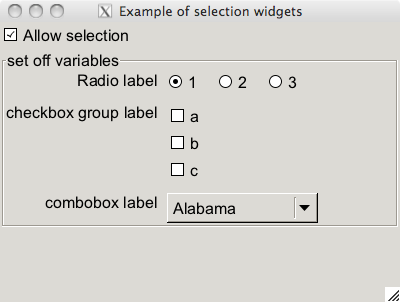
\includegraphics[width=.5\textwidth]{ex-gWidgets-selection-widgets}
  \caption{A template for a GUI using some of the widgets for selection.}
  \label{fig:ex-gWidgets-selection-widgets}
\end{figure}

This example provides template for a possible GUI that would allow a
specification of arguments for a function
(Figure~\ref{fig:ex-gWidgets-selection-widgets}).  A checkbox is
used to toggle whether the other controls are enabled or not.
\begin{Schunk}
\begin{Sinput}
 w <- gwindow("Example of selection widgets", visible=FALSE)
 g <- ggroup(horizontal=FALSE, cont=w)
 cb <- gcheckbox("Allow selection", cont=g, checked=FALSE, 
                 handler = function(h, ...) {
                   enabled(f) <- svalue(cb)
                 })
 f <- gframe("set off variables", cont=g)
 tbl <- glayout(cont=f)
 right <- c(1, 1); left <- c(-1, 1)
 tbl[1,1, anchor=right] <- "Radio label"
 tbl[1,2, anchor=left] <- (rb <- gradio(1:3, horizontal=TRUE, 
            cont = tbl))
 tbl[2,1, anchor=right] <- "checkbox group label"
 tbl[2,2, achor=left] <- (chb <- gcheckboxgroup(letters[1:3], 
            horizontal=FALSE, cont = tbl))
 tbl[3,1, anchor=right] <- "combobox label"
 tbl[3,2, achor=left] <- (combo <- gcombobox(state.name, 
            cont = tbl))
 enabled(f) <- FALSE                     
 visible(w) <- TRUE
\end{Sinput}
\end{Schunk}
               
    
\end{example}

\subsection{Display of tabular data}
\label{sec:gWidgets-tabular-data-display}


The \constructor{gtable} constructor produces a widget that displays data in a tabular form
from which the user can select one (or more) rows. The widgets
performance under \pkg{RGtk2} is much faster and able to handle larger
data stores than under \pkg{tcltk}, as there is no native table widget in \tcltk. Both perform well on moderate-sized data sets (10 or so columns and fewer than 500 rows),

The data is specified through the \argument{items}{gtable}
argument. This may be a data frame, matrix or vector. Vectors are
coerced to data frames.  The data is presented in a tabular form, with
column headers derived from the \code{names} attribute of the data
frame.  The \argument{icon.FUN}{gtable} argument is used to place a
stock icon in a left-most column.  This argument takes a function of a
single argument -- the data frame being shown -- and should return a
character vector of stock icon names, one for each row. 

\paragraph{Filtering}
The arguments \argument{filter.column}{gtable} and
\argument{filter.FUN}{gtable} allow one to specify whether the user
can filter, or limit, the display of the values in the data store. If
a column number is specified to \code{filter.column} then a combobox
is added to the widget with values taken from the unique values in the
specified column. Changing the value of the combobox, restricts the
display of the data to just those rows which match that column's
values. More advanced filtering can be specified using the
\argument{filter.FUN}{gtable} argument. If this is a function, then it takes
arguments \code{(data\_frame, filter.by)} where the data frame is the
data, and the \code{filter.by} value is the state of a combobox whose
values are specified through the argument
\argument{filter.labels}{gtable}. This function should return a logical
vector with length matching the number of rows in the data frame.
Only rows corresponding to \code{TRUE} values will be displayed. If
\code{filter.FUN} is the character string ``\code{manual}'' then the
\method{visible\ASSIGN}{gtable} method can be used to control the
filtering, again by specifying a logical vector of the proper
length. See Example~\ref{ex-gWidgets-filter-gtable} for an
application.

\paragraph{Selection}
Users can select a row, not a cell from this widget. The value returned by a selection is
controlled by the arguments \argument{chosencol}{gtable}, which
specifies which column value will be returned, as the user can only
specify the row; and \argument{multiple}{gtable} which controls
whether the user may select more than one row.  The
\method{svalue}{gtable} method will return the currently selected
value. If the argument \code{index} is specified as \code{TRUE}, then
the selected row index (or indices) will be returned. These refer to
the data store, not the visible data when filtering is being used. The
argument \code{drop} specifies if just the chosen column's value is
returned (the default) or if specified as \code{FALSE} the entire row.

\paragraph{Methods}
The underlying data store is referenced by the \method{[}{gtable}
method. Indices may be used to access just a portion. Values may be
set using the \method{[\ASSIGN}{gtable} method, but be warned it is
not as flexible as assigning to a data frame. The underlying
toolkits may not like to change the type of data displayed in a
column, so when updating a column do not assume some underlying
coercion, as is done with \R's data frames. To replace the data store, the \code{[\ASSIGN} can
be used via \code{obj[] \ASSIGN\/ new\_data\_frame}. The methods
\method{names}{gtable} and \method{names\ASSIGN}{gtable} refer to the
column headers, and \method{dim}{gtable} and \method{length}{gtable}
the underlying dimensions of the data store.

\paragraph{Handlers}
Selection is done through a single click. The \method{addHandlerClick}{gtable}
method can be used to assign a handler to those events. The default
handler is \method{addHandlerDoubleclick}{gtable}, which assigns a
handler for a double click event. Also of interest are the
\method{addHandlerRightclick}{gtable} and
\method{add3rdMousePopupMenu}{gtable} methods for assigning handlers
to  right-click events.

The \constructor{gtable} widget shows clearly the trade offs between
using \pkg{gWidgets} and a native toolkit under \R. As will be seen in later chapters,
setting up a table to display a data frame using the \pkg{RGtk2} or \pkg{tcltk} packages can involve a fair amount
of coding as compared to
\constructor{gtable}, which makes it very easy. However, there is far
less power possible from \pkg{gWidgets}. For example, there is no
method to adjust the column sizes programatically (although they can
be adjusted with the mouse),there is no means to adjust the formatting of
the displayed text, or to embed other widgets into the tabular display.

\begin{example}{Simple filtering}{ex-gWidgets-simple-filter-gtable}
  We use the \code{Cars93} data set from the \pkg{MASS} package to
  show how to set up a display of the data which provides simple
  filtering based on the type of car, whose value is stored in column 3.
  
\begin{Schunk}
\begin{Sinput}
 require(MASS)
 w <- gwindow("gtable example")
 tbl <- gtable(Cars93, chosencol=1, filter.column=3, cont=w)
\end{Sinput}
\end{Schunk}

Adding a handler for the double click event is illustrated bleow. This
handler prints both the manufacturer and the model of the currently
selected row when called.
\begin{Schunk}
\begin{Sinput}
 addHandlerChanged(tbl, handler=function(h,...) {
   val <- svalue(h$obj, drop=FALSE)
   cat(paste("You selected the", val[,1], val[,2], "\n", sep=" "))
 })
\end{Sinput}
\end{Schunk}
%%$ emacs
\end{example}


\begin{example}{More complex filtering}{ex-gWidgets-filter-gtable}
%% Example of hand-built filter using gtable

Even with moderate-sized data sets, the number of rows can be quite large, in which case it is
inconvenient to use a GUI for selection unless some means of searching or filtering the
data is used. This example uses the possible CRAN sites, to show how a
\code{gedit} instance can be used as a search box to filter the display of
data. The \code{addHandlerKeystroke} method is used so that the search
results are updated as the user types.


The \code{available.packages} function returns a data frame of all
available packages. If a CRAN site is not set, the user will be
queried to set one.
\begin{Schunk}
\begin{Sinput}
 d <- available.packages()       # pick a cran site
\end{Sinput}
\end{Schunk}

This basic GUI is barebones, for example it has no text labels to guide the user. 
\begin{Schunk}
\begin{Sinput}
 w <- gwindow("test of filter")
 g <- ggroup(cont=w, horizontal=FALSE)
 ed <- gedit("", cont=g)
 tbl <- gtable(d, cont=g, filter.FUN="manual", expand=TRUE)
\end{Sinput}
\end{Schunk}
The \argument{filter.FUN}{gtable} provides a means to have a combobox
control the display of the table. For this example, we desire more
flexibility, so we specify the value of \qcode{manual}.

Different search criteria may be desired, so it makes sense to
separate out this code from the GUI code using a function. The one below
uses \code{grep} to match, so that regular expressions can be
used. Another reasonable choice would be to use the first letter of
the package. (That filtering could also be specified easily through the
\argument{filter.FUN}{gtable} argument.)

\begin{Schunk}
\begin{Sinput}
 ourMatch <- function(curVal, vals) {
   ind <- grep(curVal, vals)             # indices
   vis <- rep(FALSE, length(vals))
   if(legnth(ind) > 0)
     vis[ind] <- TRUE
   return(vis)                           # logical
 }
\end{Sinput}
\end{Schunk}

Finally, the \code{addHandlerKeystroke} method calls its handler
everytime a key is released while the focus is in the edit widget. In
this case, the handler finds the matching indices using the
\code{ourMatch} function, converts these into logical format, and then
updates the display using the \meth{visible\ASSIGN} method for
  \code{gtable}.
\begin{Schunk}
\begin{Sinput}
 id <- addHandlerKeystroke(ed, handler=function(h, ...) {
   vals <- tbl[, 1, drop=TRUE]
   curVal <- svalue(h$obj)
   vis <- ourMatch(curVal, as.character(vals))
   visible(tbl) <- vis
 })
\end{Sinput}
\end{Schunk}
\end{example}



\subsection{An editor for tabular data}
\label{sec:gWidgets-an-editor-tabular}

The \constructor{gdf} constructor returns a  widget for editing data frames. This is similar to the GUI provided by the \code{data.entry} function, but uses the underlying toolkit in use by \pkg{gWidgets}. Each cell can be edited. Users can click (or double click) in a cell to select it, or use the arrow and \kbd{tab} keys to navigate. For \pkg{gWidgetstcltk}, there is no native widget for editing tabular data, so the \code{tktable}, add-on widget is used (\url{tktable.sourceforge.net}). A warning will be issued if this is not installed. Again, the widget under \pkg{RGtk2} is much faster than that under \pkg{tcltk}, but both can load a moderately sized data frame in a reasonable time.

The constructor has argument \argument{items}{gdf} to specify the data frame to edit and \argument{name}{gdf} to specify the data frame name, if desired. The column types are important, in particular factors and character types are treated differently, although they may render in a similar manner. 

\paragraph{Methods} Under both \pkg{RGtk2} and \pkg{tcltk} there are
bindings for right-mouse clicks that allow the user to modify the data
frame displayed. In addition, there are several methods defined that
follow those of a data frame. The \method{[}{gdf} and
\method{[\ASSIGN}{gdf} methods can be used to extract and set values
from the data frame by index. As with \code{gtable}, these are not as
flexible as for a data frame though. In particular, it may not be
possible to changes the type of a column, or add new rows or columns
through these methods. Using no indices, as in \code{obj[,]} will
return the current data frame, which can be assigned to some value for
saving. The current data frame can be completely replaced, when no
indices are specified in the replacement call. Additionally, the data
frame methods \method{dimnames}{gdf}, \method{dimnames\ASSIGN}{gdf},
\method{names}{gdf}, \method{names\ASSIGN}{gdf}, and \method{length}{gdf}
are defined.

The \constructor{gdfnotebook} constructor produces a notebook that can hold several data frames at once.

\section{Selection from a sequence of numbers}
\label{sec:gWidgets-select-from-sequ}

The previous widgets allowed selection from a user-specified set of
values. When these values are a sequence of numbers, the slider
control and spin button control are also commonly used. Both of these
widgets have arguments to specify the sequence that match those of the
\code{seq} function in \R: \argument{from}{gslider},
\argument{to}{gslider}, and \argument{by}{gslider}.

\subsection{A slider control}
\label{sec:gWidgets-slider-control}

The \constructor{gslider} constructor creates a slider that allows the
user to select a value from the specified sequence.  In
\pkg{gWidgetstcltk} the sequence must have integer steps. If this is
not the case, the spin button control is used instead. In addition to
the arguments to specify the sequence, the argument
\argument{value}{gslider} is used to set the initial value of the
widget and \argument{horizontal}{gslider} controls how the slider is
drawn, \code{TRUE} for horizontal, \code{FALSE} for vertical.

The \method{svalue}{gslider} method returns the currently chosen  value. The \method{[\ASSIGN}{gslider} method can be used to update the sequence of values to choose from.

The default handler is called when the slider is changed. Example~\ref{ex-gWidgets-sliders-spingbuttons}
shows how this can be used to update a graphic.


\subsection{A spin button control}
\label{sec:gWidgets-spin-button-control}

The spin button control constructed by \constructor{gspinbutton} is
similar to  \constructor{gslider}, but presents the user a different
way to select the value. The argument \argument{digits}{gspinbutton}
specifies how many digits are displayed. 

\begin{example}{Example of sliders and spin buttons}{ex-gWidgets-sliders-spingbuttons}
  The use of sliders and spin buttons to dynamically adjust a graphic
  is common in \R\/ GUIs targeted towards teaching statistics. Here is
  an example, similar to the \code{tkdensity} example of \pkg{tcltk},
  where the slider controls the bandwidth of a density estimation and
  the spin button the sample size of a random sample.
\begin{Schunk}
\begin{Sinput}
 w <- gwindow("Slider and Spin Button example") 
 tbl <- glayout(cont=w)
 tbl[1,1] <- "sample size"
 tbl[1,2] <- (spinner <- gspinbutton(from=10, to=100, by=5, 
                                     value=25, cont=tbl))
 tbl[2,1] <- "adjusted bandwidth"
 tbl[2,2, expand=TRUE] <- (slider <- gslider(from=0.1, to=1, 
            by=0.01, value=1, cont=tbl))
 plotGraph <- function(h,...) {
   x <- rexp(svalue(spinner))
   plot(density(x, adj=svalue(slider)))
 }
 QT <- sapply(list(spinner, slider), function(i) 
   addHandlerChanged(i, handler=plotGraph))
\end{Sinput}
\end{Schunk}
\end{example}


\section{Display of heirarchical data}
\label{sec:gWidgets-displ-heir-data}

The \constructor{gtree} constructor can be used to display
heirarchical structures, such as a file system. This constructor
parameterizes the data to be displayed in terms of the node of the
tree that is currently selected. The \argument{offspring}{gtree}
argument is assigned a function of two variables, the path in the tree
that the node in question is on and any data passed through the
optional \argument{offspring.data}{gtree} argument. This function
should return a data frame with each row referring to an offspring for
the node and whose first column is a key that characterizes the node
of the offspring, unless the argument \argument{chosencol}{gtree} is
used to specify otherwise.

To indicate if a node has offspring, a function can be passed through
the \argument{hasOffspring}{gtree} argument. This function takes the
data frame returned by the \code{offspring} function and should return
a logical vector with each value indicating which rows have
offspring. If it is more convenient to compute this within the
\code{offspring} function, then when \code{hasOffspring} is left
unspecified and the second column returned by \code{offspring} is a
logical, then that column will be used.

A single click is used to select a row. Multiple selections are
possible if the \argument{multiple}{gtree} argument is given a
\code{TRUE} value.

For some toolkits the \argument{icon.FUN}{gtree} can be used to
specify a stock icon to be displayed next to the first column. This
function, like \code{hasOffspring} has as an argument the data frame
returned by \code{offspring} and should return a character vector with
each entry indicating which stock icon is to be shown.

For some toolkits, the column type must be determined prior to
rendering. By default, a call to \code{offspring} with argument
\code{c()} indicating the root node is made. The returned data frame
is used to determine the column types. If that is not correct, the
argument \argument{col.types}{gtree} can be used. It should be a data
frame with column types matching those returned by \code{offspring}.

\paragraph{methods}
The \method{svalue}{gtree} method returns the currently selected key, or node label. There is no assignment method. The \method{[}{gtree} method returns the path for the currently node. This is what is passed to the \code{offspring} function. The method \method{addHandlerDoubleclick}{gtree} can be used to specify a function to call on a double click event.

\begin{example}{Using \code{gtree} to explore a recursive partition}{ex-gWidgets-gtree}

The \pkg{party} package implements a recursive partitioning algorithm
for tree-based regression and classification models. The package
provides an excellent \code{plot} method for the object, but in this
example we demonstrate how the \code{gtree} widget can be used to display
the heiarchical nature of the fitted object. First, we fit a model from an
example appearing in the package's vignette.

\begin{Schunk}
\begin{Sinput}
 require(party)
 data("GlaucomaM", package="ipred")      # load data
 gt <- ctree(Class ~ ., data=GlaucomaM)  # fit model
\end{Sinput}
\end{Schunk}

The \pkg{party} object tracks the heirarchical nature through its
nodes. This object if a complex structure using lists to store data
about the nodes. We define an \code{offspring} function next that
tracks the node by number, as is done in the \pkg{party} object;
records whether a node has offspring through the \code{terminal}
component (by passing the \code{hasOffspring} function); and computes
condition on the variable that creates the node. For this example, the
trees are all binary trees with 0 or 2 offspring so this data frame
has only 0 or 2 rows.

\begin{Schunk}
\begin{Sinput}
 offspring <- function(key, offspring.data) {
   if(missing(key) || length(key) < 1)  # which node?
     node <- 1
   else
     node <- as.numeric(key[length(key)]) # key is a vector
 
   if(nodes(gt, node)[[1]]$terminal)    # return if terminal
     return(data.frame(node=node, hasOffspring=FALSE,
                       description="terminal"))
 
   df <- data.frame(node=integer(2), hasOffspring=logical(2),
                    description=character(2), 
                    stringsAsFactors=FALSE)
   ## party internals
   children <-  c("left","right")
   ineq <- c(" <= "," >  ")
   varName <- nodes(gt, node)[[1]]$psplit$variableName
   splitPoint <- nodes(gt, node)[[1]]$psplit$splitpoint
 
   for(i in 1:2) {
     df[i,1] <- nodes(gt, node)[[1]][[children[i]]][[1]]
     df[i,2] <- !nodes(gt, df[i,1])[[1]]$terminal
     df[i,3] <- paste(varName, splitPoint, sep=ineq[i])
   }
   df                                    # returns a data frame
 }
\end{Sinput}
\end{Schunk}

\begin{figure}
  \centering
  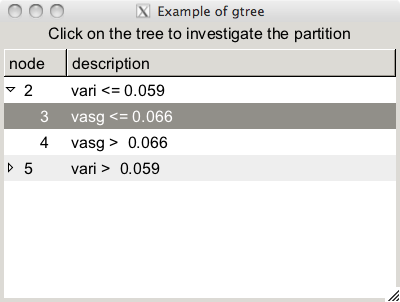
\includegraphics[width=.5\textwidth]{ex-gWidgets-gtree}
  \caption{GUI to explore return value of a model fit by the \code{party}  package.}
  \label{fig:ex-gWidgets-gtree-party}
\end{figure}


We make a simple GUI to show the widget (Figure~\ref{fig:ex-gWidgets-gtree-party})
\begin{Schunk}
\begin{Sinput}
 w <- gwindow("Example of gtree")
 g <- ggroup(cont=w, horizontal=FALSE)
 l <- glabel("Click on the tree to investigate the partition", 
             cont=g)
 tr <- gtree(offspring, cont=g, expand=TRUE)
\end{Sinput}
\end{Schunk}

A single click is used to expand the tree, here we create a binding to  a double
click event to create a basic graphic. The vignette shows how to make more
complicated -- and meaningful -- graphics for this model fit.
\begin{Schunk}
\begin{Sinput}
 addHandlerDoubleclick(tr, handler=function(h,...) {
   node <- as.numeric(svalue(h$obj))
   if(nodes(gt, node)[[1]]$terminal) {   # if terminal plot
     weights <- as.logical(nodes(gt,node)[[1]]$weights)
     plot(response(gt)[weights, ])
   }})
\end{Sinput}
\end{Schunk}
\end{example}

\section{Selecting from the file system}
\label{sec:gWidgets-selecting-from-file}

The \constructor{gfile} dialog allows one to select a file or directory
from the file system. This is a modal dialog, which returns the name
of the selected file or directory. The \constructor{gfilebrowse}
constructor creates a widget that has a button that allows the user to
initiate this selection.  

The selection type is specified by the \code{type} argument with
values of \code{open}, to select an existing file; \code{save} to select a file
to write to; and \code{selectdir} to select a directory. For
\code{RGtk2}, the \argument{filter}{gfile} argument can be used to
narrow the listed files. The dialog returns the path of the file, or \code{NA} if the dialog was canceled. One can also
specify a handler to the constructor to call on the file or directory
name. The component \code{file} of the first argument to the handler
contains the file name.

\begin{Schunk}
\begin{Sinput}
 if(!is.na(tmp <- gfile())) 
   source(tmp)
 ## or
 gfile(handler=function(h,...) {
   if(!is.na(h$file))
     source(h$file) 
 })   
\end{Sinput}
\end{Schunk}
%$


\subsection{Selecting a date}
\label{sec:gWidgets-selecting-date}

The \constructor{gcalendar} constructor returns a widget that can be
used to select a date if the underlying toolkit supports such a widget
or a text edit box to allow the user to enter a date. The argument
\argument{text}{gcalendar} arugment can used to specify the initial
text. The \argument{format}{gcalendar} is used to specify the format of the date.

The methods for the widget inherit from \code{gedit}. In particular,
the \method{svalue}{gcalendar} method returns the text in the text box
as a character vector formatted by the value specified by the
\argument{format}{gcalendar} argument. To return a value of a
different class, pass a function, such as \code{as.Date} to the
\argument{coerce.with}{gcalendar} argument.


\section{Display of graphics}
\label{sec:gWidgets-display-grapics}

\subsection{Displaying icons and images store in files}
\label{sec:gWidgets-displ-icons-imag}

Graphics files can be displayed by the \constructor{gimage}
widget. (Not all file types may be displayed by each toolkit, in
particular \pkg{gWidgetstcltk} can only display gif, ppm, and xbm
files.)  The file to display is specified through the
\argument{filename}{gimage} argument of the constructor. This value is combined with that
of the \argument{dirname}{gimage} argument to specify the file
path. 

The \pkg{gWidgets} package provides a few stock icons, that simplify
the above.  Stock icons, can be specified by using their name for the
\code{filename} argument and the character string \code{"stock"} for
the \code{dirname} argument. A list of the defined stock icons is
returned by the function \code{getStockIcons}. The names attribute
defines the valid stock icon names.  For \pkg{gWidgetsRGtk2}, the size
of a stock icon can be adjusted through the \argument{size}{gimage} argument,
with a value from \qcode{menu}, \qcode{small\_toolbar},
\qcode{large\_toolbar}, \qcode{button}, or \qcode{dialog}.

%% methods

The \method{svalue\ASSIGN}{gimage} method can be used to change the
graphics file. In this case, a full path name is specified, or the
stock icon name.


More stock icon names may be added through the function
\code{addStockIcons}. This function requires a vector of stock icon
names and a vector of corresponding file paths, and is illustrated in
the example.

%% handlers
The default handler is called on a click event.

\begin{example}{Adding and using stock icons}{ex-gWidgets-stock-icons}
This example shows how to add to the available stock icons and use
\code{gimage} to display them. It creats a table to select a color
from, as an alternative to a more complicated color chooser dialog. Under \pkg{gWidgetstcltk} the image
files would need to be converted to \code{gif} format, as \code{png}
format is not a natively supported image type. 

We begin by defining 16 arbitrary colors.

\begin{Schunk}
\begin{Sinput}
 someColors <- c("black", "red", "blue", "brown",
                 "green", "yellow", "purple",
                 paste("grey", seq(10,90,by=10), sep=""))
\end{Sinput}
\end{Schunk}

This is the function that is used to create an icon file. We use some
low-level \pkg{grid} functions to draw the image to a png file.
\begin{Schunk}
\begin{Sinput}
 require(grid)
 iconDir <- tempdir(); iconSize <- 16;
 makeColorIcon <- function(i) {
   filename <- paste(iconDir, "/color-", i, ".png",
                     sep="", collapse="")
   png(file=filename, width=iconSize, height=iconSize)
   grid.newpage()
   grid.draw(rectGrob(gp=gpar(fill=i)))
   dev.off()
   return(filename)
 }
\end{Sinput}
\end{Schunk}

To add icons, we need to define the stock names and the file paths for
\code{addStockIcons}.

\begin{Schunk}
\begin{Sinput}
 icons <- sapply(someColors, makeColorIcon)
 iconNames <- paste("color-", someColors, sep="")
 QT <- addStockIcons(iconNames, icons)
\end{Sinput}
\end{Schunk}

We use a table layout to show the 16 colors. As an illustration of
assigning a handler for a click event, we assign one that returns the
corresponding stock icon name.

\begin{Schunk}
\begin{Sinput}
 w <- gwindow("Icon example")
 f <- function(h,...) print(h$action)
 tbl <- glayout(cont = w, spacing=0)
 for(i in 1:4) {
   for(j in 1:4) {
     ind <- (i - 1) * 4 + j
     tbl[i,j] <- gimage(icons[(i-1)*4 + j], handler=f, 
                        action=iconNames[ind], cont=tbl)
   }
 }
\end{Sinput}
\end{Schunk}
\end{example}

\subsection{A graphics device}
\label{sec:gWidgets-graphics-device}

Some toolkits support an embeddable graphics device (\pkg{RGtk2}
through \pkg{cairoDevice}). In which case, the \constructor{ggraphics}
constructor produces a widget that can be added to a container. The
arguments \argument{width}{ggraphics}, \argument{height}{ggraphics},
\argument{dpi}{ggraphics}, \argument{ps}{ggraphics} are similar to
other graphics devices.

The \constructor{ggraphicsnotebook} creates a notebook that allows the
user to easily navigate multiple graphics devices.


%%% 
\begin{example}{A GUI to explore a data set}{ex-gWidgets-baseball}
\begin{Schunk}
\begin{Soutput}
The  hash  package provided by:
                            _       _        
  ___  _ __   ___ _ __   __| | __ _| |_ __ _ 
 / _ \| '_ \ / _ \ '_ \ / _` |/ _' | __/ _' |
| (_) | |_) |  __/ | | | (_| | (_| | || (_| |
 \___/| .__/ \___|_| |_|\__,_|\__,_|\__\__,_|
      |_|   http://www.opendatagroup.com      
\end{Soutput}
\end{Schunk}

\begin{figure}
  \centering
  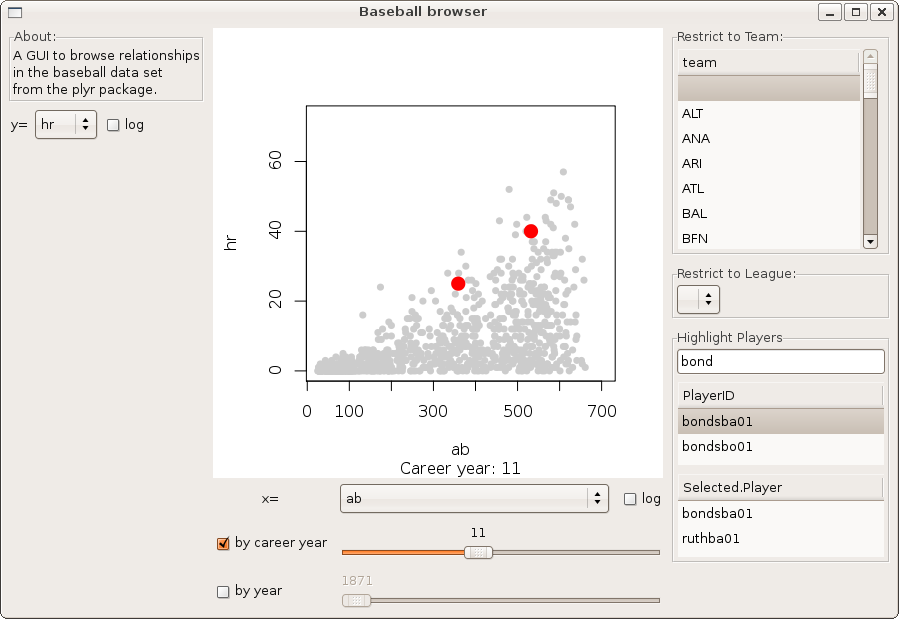
\includegraphics[width=.8\textwidth]{fig-gWidgets-baseball-gui.png}
  \caption{A \pkg{RGtk2} GUI for exploring the \code{baseball} data set of the \code{plyr} package. One can subset by year or career year through the slider widgets.}
  \label{fig:ex-gWidgets-baseball}
\end{figure}

This example creates a GUI to explore the \code{baseball} data set of
the \pkg{plyr} package.  The baseball data set contains information by
year for players who had 15-year or longer careers. Several
interesting things can be seen by looking at specific players, such as
Babe Ruth (coded \code{ruthba01}) or Barry Bonds (\code{bondsba01}).
Before beginning, we follow an example from the \pkg{plyr} package to create a
new variable to hold the career year of a player.
\begin{Schunk}
\begin{Sinput}
 data(baseball, package="plyr")
 calc <- function(df) 
   transform(df,
             cyear = year - min(year),
             cpercent = (year - min(year))/(max(year) - min(year)))
 b <- ddply(baseball, .(id), calc)
 b <- subset(b, ab >= 25) 
 nVars <- names(b)[-c(1:5,23:24)]    # numeric variables
\end{Sinput}
\end{Schunk}

This example uses the \pkg{hash} package to store our data and an environment to store our widgets.
\begin{Schunk}
\begin{Sinput}
 require(hash)
 dat <- hash()
 e <- new.env()
\end{Sinput}
\end{Schunk}

The following function transfers values from the GUI to our data
store, \code{dat}, returning \code{TRUE} if all goes well. The widgets
are all stored in an environmen, \code{e} below, using names which
are again used as keys to the hash. We also define a function
\code{plotIt} to produce a graphic based on the current state of the
data store, but don't reproduce it here.
\begin{Schunk}
\begin{Sinput}
 transferData <- function() {
   out <- try(sapply(e, svalue, drop=TRUE), silent=TRUE)
   if(inherits(out,"try-error"))
     return(FALSE)
   dat[[names(out)]] <- out              # hash keys
   dat$id <- e$id[]                      # not svalue
   return(TRUE)                          # works!
 }
\end{Sinput}
\end{Schunk}


We now create a GUI so that the user can select which graphic to
make. Our GUI will have a main plot window to show a scatter plot, and
controls to adjust the variables that are plotted, and to filter that
values plotted. 

Our layout will use box containers to split the top-level window into
three panes. The middle one holds the graphic, so we set it to
\code{expand} when the window is resized.
\begin{Schunk}
\begin{Sinput}
 w <- gwindow("Baseball browser", visible=FALSE)
 g <-  ggroup(cont=w, horizontal=TRUE)
 lp <- ggroup(cont=g, horizontal=FALSE)
 cp <- ggroup(cont=g, horizontal=FALSE, expand=TRUE)
 rp <- ggroup(cont=g, horizontal=FALSE, spacing=10)
\end{Sinput}
\end{Schunk}

The left panel holds a short description and a combobox to select the $y$-variable plotted.
\begin{Schunk}
\begin{Sinput}
 f <- gframe("About:", cont=lp)
 l <- glabel(paste("A GUI to browse relationships",
              "in the baseball data set",
              "from the plyr package.",
              sep="\n"),
        cont=f)
 g1 <- ggroup(cont=lp)
 l <- glabel("y=", cont=g1)
 e$y <- gcombobox(nVars, selected=4, cont=g1)
 e$ylog <- gcheckbox("log", checked=FALSE, cont=g1)
\end{Sinput}
\end{Schunk}

The center panel holds the \code{ggraphics} object, along wtih controls
to select the $x$ variable. As well, we add controls to filter out the
display by either the year a player played and/or their career year. A \code{gtable} instance is used for layout.
\begin{Schunk}
\begin{Sinput}
 gg <- ggraphics(cont=cp)
 tbl <- glayout(cont=cp)
 tbl[1,1] <- "x="
 tbl[1,2, expand=TRUE] <- (e$x <- gcombobox(nVars, selected=2, 
            cont=tbl))
 tbl[1,3] <- (e$xlog <- gcheckbox("log", checked=FALSE, 
                                  cont=tbl))
 ##
 tbl[2,1] <- (e$doCareerYear <- gcheckbox("by career year", 
                                          checked=TRUE, cont=tbl))
 tbl[2,2:3, expand=TRUE] <- (e$cyear <- 
              gslider(min(b$cyear), max(b$cyear), by=1, cont=tbl))
 enabled(e$cyear) <- TRUE
 ##
 tbl[3,1] <- (e$doYear <- gcheckbox("by year", 
                                    checked=FALSE, cont=tbl))
 tbl[3,2:3, expand=TRUE] <- (e$year <- 
              gslider(min(b$year), max(b$year), by=1, cont=tbl))
 enabled(e$year) <- FALSE
\end{Sinput}
\end{Schunk}

The right panel includes a few means to filter the display of
values. We use a simple \code{gtable} widget to allow the user to
restrict the display to one or more teams. A combobox allows the user
to restrict to one of the historic leagues. To allow certain players
to stand out, a compound widget is made using a \code{gedit} object to
filter values, a \code{gtable} object to show all possible IDs, and a
\code{gtable} object to show the selected IDs to highlight. Frame are
used to visually combine these controls.
\begin{Schunk}
\begin{Sinput}
 rpWidth <- 200
 f <- gframe("Restrict to Team:", cont = rp)
 teams <- data.frame(team=c("", sort(unique(b$team))), 
                     stringsAsFactors=FALSE)
 e$team <- gtable(teams, cont=f, multiple=TRUE, width=rpWidth)
 size(e$team) <- c(200,200)
 svalue(e$team, index=TRUE) <- 1
 ##
 f <- gframe("Restrict to League:", cont=rp)
 leagues <- names(table(b$lg))[-1]       # drop ""
 e$lg <- gcombobox(c("", leagues), cont=f)
 ##
 f <- gframe("Highlight Players", horizontal=FALSE, cont=rp)
 searchPlayer <- gedit("", cont=f)
 listPlayers <- gtable(data.frame("PlayerID"=unique(b$id), 
                                  stringsAsFactors=FALSE),
                       filter.FUN="manual", cont=f)
 e$id <- gtable(data.frame("Selected Player"=character(0), 
                           stringsAsFactors=FALSE), cont=f)
\end{Sinput}
\end{Schunk}

We define several handlers to make the GUI responsive to user
output. Rather than write an \code{updateUI} function to update the
GUI at periodic intervals, we use an event-driven model. These first
two handlers, simply toggle whether the user can control the display
by year or career year.
\begin{Schunk}
\begin{Sinput}
 addHandlerChanged(e$doYear, handler = function(h,...) {
   val <- ifelse(svalue(e$doYear), TRUE, FALSE)
   enabled(e$year) <- val
 })
 addHandlerChanged(e$doCareerYear, handler = function(h,...) {
   val <- ifelse(svalue(e$doCareerYear), TRUE, FALSE)
   enabled(e$cyear) <- val
 })
\end{Sinput}
\end{Schunk}
This next handler updates the graphic when any of several widgets is changed.
\begin{Schunk}
\begin{Sinput}
 QT <- sapply(list(e$x, e$xlog, e$y, e$ylog, e$year, e$cyear,
                   e$doYear, e$doCareerYear, e$lg), function(i)
              addHandlerChanged(i, handler=function(h, ...) 
                                transferData() && plotIt()))
\end{Sinput}
\end{Schunk}

For \code{gtable} objects, it is more natural here to bind to a single
mouse click, rather than the default double click.

\begin{Schunk}
\begin{Sinput}
 QT <- sapply(list(e$team, e$id), function(i)
        addHandlerClicked(i, handler=function(h, ...) 
                          transferData() && plotIt()))
\end{Sinput}
\end{Schunk}
These handlers are used to select the  IDs to highlight.
\begin{Schunk}
\begin{Sinput}
 addHandlerKeystroke(searchPlayer, handler=function(h, ...) {
   cur <- svalue(h$obj)
   ind <- grep(cur, unique(b$id))
   tmp <- rep(FALSE, length(unique(b$id)))
   if(length(ind) > 0) {
     tmp[ind] <- TRUE
     visible(listPlayers) <- tmp
   } else if(length(grep("^\\s$", cur))) {
     visible(listPlayers) <- !tmp
   } else {
     visible(listPlayers) <- tmp
   }
 })
 addHandlerChanged(listPlayers,handler=function(h, ...) {
   val <- svalue(h$obj)
   e$id[] <- sort(c(val, e$id[]))
 })
 addHandlerChanged(e$id, handler=function(h, ...) {
   val <- svalue(h$obj)
   cur <- e$id[]
   e$id[] <- setdiff(cur, val)
 })
\end{Sinput}
\end{Schunk}

Finally, we implement functionality similar to the \code{locator}
function for the graphic. This handler labels the point nearest to a mouse click in
the plot area.
\begin{Schunk}
\begin{Sinput}
 distance <- function(x,y)  {
   ds <- apply(y, 1, function(i) sum((x-i)^2))
   ds[is.na(ds)] <- max(ds, na.rm=TRUE)
   ds
 }
 addHandlerClicked(gg, function(h,...) {
   x <- c(h$x, h$y)
   ds <- distance(x, curdf[,2:3])
   ind <- which(ds == min(ds))
   ids <- curdf[ind, 1]
   points(y[ind,1], y[ind,2], cex=2, pch=16, col="blue")
   text(y[ind,1], y[ind,2], label=ids, adj=c(-.25,0))
 })
\end{Sinput}
\end{Schunk}

To end, we show the GUI and initialize the plot.
\begin{Schunk}
\begin{Sinput}
 visible(w) <- TRUE
 QT <- transferData() && plotIt()
\end{Sinput}
\end{Schunk}
\end{example}


\section{Dialogs}
\label{sec:gWidgets-modal-dialogs}

The \pkg{gWidgets} package provides a few constructors to quickly make
some basic  dialogs for showing messages or gathering
information. Mostly these are modal dialogs that take control of the
eventloop, not allowing any other part of the GUI to be active for
programmatic interaction. As such, the constructors do not return an
object to manipulate through its methods, but rather the value of the
dialog specified by the user. Hence, they are used differently than
other constructors. For example, the \code{gfile} dialog, previously described, is
a modal dialog that pops up a means to select a file returning
the selected file path or \code{NA}.


\begin{table}
\centering
\label{tab:gWidgets-basic-dialogs}
\caption{Table of constructors for basic dialogs in \pkg{gWidgets}}
\begin{tabular}{@{}lp{0.7\textwidth}@{}}
\toprule

Constructor&Description\\
\midrule
\constructor{gfile}&File and directory selection dialog\\\constructor{gmessage}&Dialog to show a message\\\constructor{galert}&Unobtrusive (non-modal) dialog to show a message\\\constructor{gconfirm}&Confirmation dialog\\\constructor{ginput}&Dialog allowing user input\\\constructor{gbasicdialog}&Flexible modal dialog
\\ \bottomrule
\end{tabular}
\end{table}% \begin{table}
%   \centering
%  \begin{tabular}{l@{\quad}p{.75\textwidth}}
% %   \toprule
%     \constructor{gfile} & File and directory selection dialog\\
%     \constructor{gmessage} & Dialog to show a message\\
%     \constructor{galert} & Unobtrusive (non-modal) dialog to show a message\\
%     \constructor{gconfirm} & Confirmation dialog\\
%     \constructor{ginput} & Dialog allowing user input\\
%     \constructor{gbasicdialog} & Flexible modal dialog \\
%     \bottomrule
%   \end{tabular}
%   \caption{Table of basic dialogs in \pkg{gWidgets}}
%   \label{tab:gWidgets-modal-dialogs}
% \end{table}

The dialogs pop up a window with a common appearance. The
constructors have arguments \argument{message}{gmessage} for a
message; \argument{title}{gmessage} for the window title; and
\argument{icon}{gmessage} to specify an icon, whose value is one of
\qcode{info}, \qcode{warning}, \qcode{error}, or
\qcode{question}. Buttons will appear at the bottom of the dialog,
and are determined by choice of the constructor. The
\argument{parent}{gmessage} argument will place the dialog near the
\pkg{gWidgets} instance specified. Otherwise, placement will be
controlled by the window manager.

The dialogs, except for \code{galert}, have the standard
\code{handler} and \code{action} arguments, for calling a handler, but
typically it is easier to use the return value when programming.

\paragraph{A message dialog}
The simplest dialog is produced by \code{gmessage}, which is used to
display a message. The user has a cancel button to dismiss the dialog.

\paragraph{An alert dialog}
The \code{galert} dialog is similar to \code{gmessage} only it is meant
to be less obtrusive, so it is non-modal. It does not take the focus and vanishes after a time delay.

\paragraph{A confirmation dialog}
The constructor \constructor{gconfirm} produces a dialog that allows
the user to confirm the message. This dialog returns \code{TRUE} or
\code{FALSE} depending on the user's selection.


\paragraph{An input dialog}
The \constructor{ginput} constructor produces a dialog which allows
the user to input a single line of text. If the user confirms the
dialog, the value of the string is returned, otherwise if the user
cancels the dialog through the button a value of \code{NA} is returned.




\paragraph{A basic dialog}
The \constructor{gbasicdialog} constructor allows one to place an
arbirary widget within a modal window with \kbd{OK} and
\kbd{Cancel}. The handler, if specified, will be called if the user
clicks the \kbd{OK} button. This allows users to create their own
modal dialogs.

As with the others, the argument \argument{title}{gbasicdialog} is
used to specify the window title, but there is no \code{icon} or
\code{message} arguments, as there is no standard appearance. Rather,
the \argument{widget}{gbasicdialog} argument specifies a widget to
pack into the dialog. This can be a simple control, or a container
containing other widgets. 

As with \code{gconfirm}, this widget returns \code{TRUE} or
\code{FALSE} depending on the user's selection. To do something more complicated than \code{gconfirm}, a handler should be specified at construction. If the user selects
\kbd{OK}, the handler, if specified, is called before the value \code{TRUE}
is returned. 

This dialog is called a bit awkwardly, to allow it to work when controls need a
parent container specified at construction time (e.g., \pkg{tcltk}). The construction is in
three stages: an initial call to \code{gbasicdialog} to return a container which is used as
the parent container for a child component; a construction of the dialog; then a call to the
\code{visible} method on the dialog with \code{set=TRUE} value (not though \code{visible(obj) \ASSIGN\/ TRUE}).


\begin{example}{Modal dialogs}{ex-gWidgets-modal-dialogs}
The basic input dialog requires just the first argument.
\begin{Schunk}
\begin{Sinput}
 ginput("Message goes here", title="example dialog")
\end{Sinput}
\end{Schunk}

Here we use the question icon for a confirmation dialog, as the message is a question.
\begin{Schunk}
\begin{Sinput}
 ret <- gconfirm("Really delete file?", icon="question")
\end{Sinput}
\end{Schunk}

This illustrates how to use the return value.
\begin{Schunk}
\begin{Sinput}
 ret <- ginput("Enter your name", icon="info")
 if(!is.na(ret)) 
   cat("Hello",ret,"\n")
\end{Sinput}
\end{Schunk}

The \code{gbasicdialog} constructor can be used to make modal
dialogs. This example will force the user to
select a color before proceeding with anything else. 
\begin{Schunk}
\begin{Sinput}
 ## create a parent container
 dlg <- gbasicdialog("Pick a color", handler = 
                     function(h,...) print(svalue(widget)))
 ## create the dialog using dlg as the parent container
 widget <- gtable(colors(), cont = dlg)
 ## show the modal dialog (not visible(dlg) <- TRUE)
 visible(dlg, set=TRUE)    
\end{Sinput}
\end{Schunk}

\end{example}
















\section{\pkg{gWidgets}: Compound widgets}
\label{sec:compound-widgets}
The \pkg{gWidgets} package provides some \R\/ specific widgets for
producing GUIs. Table~\ref{tab:gWidgets-compound-widgets} lists them.


\begin{table}
\centering
\label{tab:gWidgets-compound-widgets}
\caption{Table of constructors for compound widgets in \pkg{gWidgets}}
\begin{tabular}{@{}lp{0.7\textwidth}@{}}
\toprule

Constructor&Description\\
\midrule
constructor{gvarbrowser}&GUI for browsing variables in the workspace\\constructor{ghelp}&GUI for a help page\\constructor{ghelpbrowser}&A help browser\\\constructor{gcommandline}&Command line widget\\constructor{gformlayout}&Uses list to specify layout of a GUI\\constructor{ggenericwidget}&Creates a GUI for a function based on its formal arguments or a defining list
\\ \bottomrule
\end{tabular}
\end{table}
% \begin{table}
%   \centering
%   \begin{tabular}{l@{\quad}p{.75\textwidth}}
% %    \toprule
%     \constructor{gcommandline} & Command line widget\\ 
%     \constructor{gvarbrowser} & GUI for browsing variables in the workspace\\
% %    \constructor{gdfnotebook} & A notebook of data frames\\
% %    \constructor{ggraphicsnotebook} & A notebook for graphics objects\\
%     \constructor{ghelp} & GUI for a help page\\
%     \constructor{ghelpbrowser} & A help browser\\
%     \constructor{gformlayout} & Uses list to specify layout of a GUI\\
%     \constructor{ggenericwidget} & Creates a GUI for a function based
%     on its formal arguments or a defining list\\
%     \bottomrule
%   \end{tabular}
%   \caption{Table of compound widgets provided by \pkg{gWidgets}}
%   \label{tab:gWidgets-compound-widgets}
% \end{table}


\subsection{Workspace browser}
\label{sec:gWidgets-workspace-browser}

A workspace browser is constructed by \code{gvarbrowser}, providing a
means to browse and select the objects in the current global environment. The
quality of the implementation varies depending on the toolkit. The
default \code{handler} object calls \code{do.call} on the object for
the function specified through the \argument{action}{gvarbrowser}
argument. The default is to print a \code{summary} of the object. This
handler is called on a double click. A single click is used for
selection. The name of the currently selected value is returned by the
\method{svalue}{gvarbrowser} method.

\subsection{Help browser}
\label{sec:gWidgets-help-browser}

The \constructor{ghelp} constructor produces a widget for showing help
pages using a notebook container. This widget does not use the html
help pages or the chm help pages, so it may not work for all operating
systems. (For Windows, the help browser of the GUI is much better
anyways.) To add a help page, the \method{add}{ghelp} method is used,
where the \code{value} argument describes the desired page. This can
be a character string containing the topic, a character string of the
form \code{package:::topic} to specify the package, or a list with
named components \code{package} and \code{topic}.  The
\method{dispose}{ghelp} method of notebooks can be used to remove the
current tab.

The \constructor{ghelpbrowser} constructor produces a stand-alone
GUI for displaying help pages, running examples from the help pages or
opening vignettes provided by the package. This GUI provides its own
top-level window and does not return a value for which methods are defined.



\subsection{Command line widget}
\label{sec:gWidgets-command-line-widget}

A simple command line widget is created by the
\constructor{gcommandline} constructor. This is not meant as a
replacement for \R's typical commandlines, but is there for
lightweight usage. A text box allows users to to type in \R\/
commands. The programmer may issue commands to be evaluated and
displayed through the \method{svalue\ASSIGN}{gcommandline} method. The
\code{value} assigned is a character string holding the commands. If
there is a names attribute, the results will be assigned to a variable
in the global workspace with that name. The \code{svalue} and \code{[}
methods return the command history.

\subsection{Simplifying creation of dialogs}
\label{sec:gWidgets-designing-forms}

The \pkg{gWidgets} package has two means to simpify the creation of
GUIs. The \code{gformlayout} constructor takes a list defining a
layout and produces a GUI, the \code{ggenericwidget} constructor can
take a function name and produce a GUI based on the formal arguments
of the function. This too uses a list, that can be modified by the
user before the GUI is constructed. 

\subsubsection{Laying out a form}
\label{sec:gWidgets-laying-out-form}

The \constructor{gformlayout} constructor takes a list defining a
layout and creates the specified widgets. The design borrows from the
\code{extjs} javascript libraries for web programming, where a similar
function can be used to specify the layout of web forms. Several
toolkits have a means to specify a layout using XML (eg. glade), this
implementation uses a list, assuming this is more familiar to the \R\/
user. By defining the layout ahead of time, pieces of the layout can
be recycled for other layouts.


To define the layout, each component is specified using a list with
named components. The component \code{type} specifies what component
to be created, as a string. This can be a the name of a container
constructor, a widget constructor or the special value
\code{"fieldset"}. Field sets are used to group a set of common
controls. If the component \code{name} is specified, then the
component that is created will be stored in the list returned by the
\code{[} method.

The \code{label} component can be specified to
add a descriptive label to the layout. When specified, the component
\code{label.pos} can be specified with value \code{"top"} to have the label
on top of the widget, or \code{"side"} to place the label on the side
(the default positioning). The \code{label.font} component can be used
to specify the label's font properties using a label's \meth{font\ASSIGN} method.

If the type is a container or
fieldset, then the \code{children} component is a list whose
components specify the children as above. Except for fieldsets, these
children can contain other containers or components. Fieldsets only
allow components as children.

Whether a widget is enabled or not can be controlled by specifying
values for \code{depends.on}, \code{depends.FUN}, and
\code{depends.signal}. If the component \code{depends.on} specifies
the name of a previous component, then the function \code{depends.FUN}
will be consulted when the signal specified by \code{depends.signal}
is emitted. This uses the \code{addHandlerXXX} names with a default
value of \code{addHandlerChanged}. The \code{depends.FUN} function has
a single argument consisting of the value returned by \code{svalue}
when called on the widget specified through \code{depends.on}. This
function should return a logical indicating if the widget is enabled
or not.

\paragraph{Methods}
The constructor returns an object with a few methods. The
\method{[}{gformlayout} method will return a list with
components being the widgets that were named in the defining list. The
\method{svalue}{gformlayout} method simply applies the \code{svalue}
method for each component of the list returned by the \code{[}
method. The \method{names}{gformlayout} method returns the names of the widgets in the list.


\begin{example}{The \code{gformlayout} constructor}{ex-gWidgets-gformlayou}
This example uses \code{gformlayout} to make a GUI for a $t$-test (Figure~\ref{fig:ex-gWidgets-formlayout}). The
first task is to define the list that will set up the GUI. We do this
in pieces. This first piece will define the part of the GUI where the
null and alternative hypotheses are specified. The null is specified
as a numeric value with a default of 0. We use the \code{gedit} widget
which by default will return a character value, so the
\code{coerce.with} argument is specified. For the alternative, this
requires a selection for just 3 possibilities, so a combo box is
employed.
\begin{figure}
  \centering
  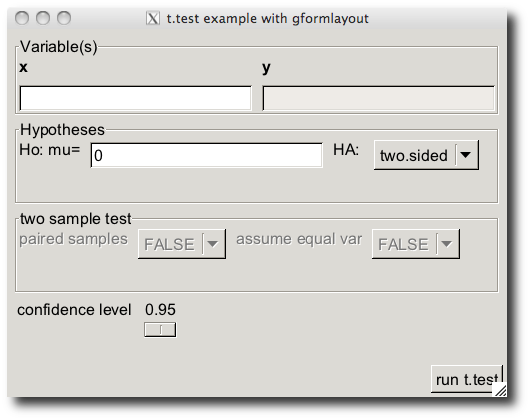
\includegraphics[width=.5\textwidth]{ex-gWidgets-formlayout}
  \caption{A dialog to collect arguments for a $t$-test made with \code{gformlayout}.}
  \label{fig:ex-gWidgets-formlayout}
\end{figure}


\begin{Schunk}
\begin{Sinput}
 hypotheses <- 
   list(type = "fieldset",
        label = "Hypotheses",
        columns = 2, 
        children = list(
          list(type="gedit",                            
               name="mu", label="Ho: mu=",
               text="0", coerce.with=as.numeric),
          
          list(type="gcombobox",
               name="alternative", label="HA: ",
               items=c("two.sided","less","greater")
               )))
\end{Sinput}
\end{Schunk}

Basic usage of the \code{t.test} function allows for an \code{x}, or
\code{x} and \code{y} variable to be specified. Here we disable the
\code{y} variable until the \code{x} one has been entered. The
\code{addHandlerChanged} method is called when the enter key is
pressed after the \code{x} value is specified.

\begin{Schunk}
\begin{Sinput}
 variables <- 
   list(type="fieldset",
        columns = 2,
        label = "Variable(s)",
        label.pos = "top",
        label.font = c(weight="bold"),
        children = list(
          list(type = "gedit",
               name = "x", label = "x",
               text = ""),
          list(type = "gedit",
               name = "y", label = "y",
               text = "",
               depends.on = "x",
               depends.FUN = function(value) nchar(value) > 0,
               depends.signal = "addHandlerChanged"
               )))
\end{Sinput}
\end{Schunk}

If a \code{y} value is specified, then the two-sample options make sense. This enables them dependent on that happening.

\begin{Schunk}
\begin{Sinput}
 two.sample <-  
   list(type = "fieldset",
        label = "two sample test",
        columns = 2,
        depends.on = "y",
        depends.FUN = function(value) nchar(value) > 0,
        depends.signal = "addHandlerChanged",                     
        children = list(
          list(type = "gcombobox",
               name = "paired", label = "paired samples",
               items = c(FALSE, TRUE)
               ),
          list(type = "gcombobox",
               name = "var.equal", label = "assume equal var",
               items = c(FALSE, TRUE)
               )))
\end{Sinput}
\end{Schunk}

The confidence interval specification is specified using a slider for variety.

\begin{Schunk}
\begin{Sinput}
 conf.level <- 
   list(type = "fieldset",
        columns = 1,
        children = list(
          list(type = "gslider",
               name = "conf.level", label = "confidence level",
               from=0.5, to=1.0, by=.01, value=0.95
               )))
\end{Sinput}
\end{Schunk}
Finally, the constituent pieces are placed inside a box container.
\begin{Schunk}
\begin{Sinput}
 tTest <- list(type = "ggroup",
               horizontal = FALSE,
               children = list(
                 variables,
                 hypotheses,
                 two.sample,
                 conf.level
                 ))
\end{Sinput}
\end{Schunk}

The layout of the GUI is primarily done by the \code{gformlayout}
call. The following just places the values in a top-level window and adds a
button to initiate the call to \code{t.test}.

\begin{Schunk}
\begin{Sinput}
 w <- gwindow("t.test example with gformlayout")
 g <- ggroup(horizontal=FALSE, cont=w)
 fl <- gformlayout(tTest, cont=g, expand=TRUE)
 bg <- ggroup(cont=g)
 addSpring(bg)
 b <- gbutton("Run t.test", cont=bg)
\end{Sinput}
\end{Schunk}

The handler is very simple, as the names chosen match the argument
names of \code{t.test}, so the list returned by the \meth{svalue}
method can be used with \code{do.call}. The only needed adjustment is
for the one-sample case.

\begin{Schunk}
\begin{Sinput}
 addHandlerChanged(b, function(h, ...) {
   out <- svalue(fl)
   out$x <- svalue(out$x) # turns text string into numbers
   if(out$y == "") {
     out$y <- out$paired <- NULL 
   } else {
    out$y <- svalue(out$y)
   }
   print(do.call("t.test", out))
 })
\end{Sinput}
\end{Schunk}

\end{example}

\subsubsection{Automatically creating a GUI}
\label{sec:gWidgets-autom-creat-gui}

The \constructor{ggenericwidget} constructor can create a basic GUI
for a function using the function's formal arguments as a guide for
the proper widget to use to collect values for an argument of the
function. The \pkg{fgui} package provides a similar function using
just the \pkg{tcltk} package, only it improves \code{ggenericwidget} by
parsing the function's help page.

The implementation actually has two stages, the first creates a list
specifying the layout of the GUI and the second a call to layout the
GUI. This list is different from that used by \code{gformlayout}. It
does not provide as much flexibility and is described in the help page
for \code{ggenericwidget}. This list can be edited if desired and then
used directly.

The formal arguments of an S3 method may be different from those of
its generic. For instance, those for the \code{t.test} generic are
much different (and less useful for this purpose) than the
\code{t.test.default} method for numeric values for \code{x}. Knowing
this, a useful GUI can be quickly created for the \code{t.test} with
the commands:
\begin{Schunk}
\begin{Sinput}
 w <- gwindow("t.test through ggenericwidget")
 f <- stats:::t.test.default; 
 widget <- ggenericwidget("f", cont=w)
\end{Sinput}
\end{Schunk}



\XXX{Need to have an example with drag and drop}


%\section{End of chapter notes}
%\label{sec:gWidgets:eoc}





